%%%%%%%%%%%%%%%%%%%%%%%%%%%%%%%%%%%%%%%%%
% University Assignment Title Page 
% LaTeX Template
% Version 1.0 (27/12/12)
%
% This template has been downloaded from:
% http://www.LaTeXTemplates.com
%
% Original author:
% WikiBooks (http://en.wikibooks.org/wiki/LaTeX/Title_Creation)
%
% License:
% CC BY-NC-SA 3.0 (http://creativecommons.org/licenses/by-nc-sa/3.0/)
% 
% Instructions for using this template:
% This title page is capable of being compiled as is. This is not useful for 
% including it in another document. To do this, you have two options: 
%
% 1) Copy/paste everything between \begin{document} and \end{document} 
% starting at \begin{titlepage} and paste this into another LaTeX file where you 
% want your title page.
% OR
% 2) Remove everything outside the \begin{titlepage} and \end{titlepage} and 
% move this file to the same directory as the LaTeX file you wish to add it to. 
% Then add %%%%%%%%%%%%%%%%%%%%%%%%%%%%%%%%%%%%%%%%%
% University Assignment Title Page 
% LaTeX Template
% Version 1.0 (27/12/12)
%
% This template has been downloaded from:
% http://www.LaTeXTemplates.com
%
% Original author:
% WikiBooks (http://en.wikibooks.org/wiki/LaTeX/Title_Creation)
%
% License:
% CC BY-NC-SA 3.0 (http://creativecommons.org/licenses/by-nc-sa/3.0/)
% 
% Instructions for using this template:
% This title page is capable of being compiled as is. This is not useful for 
% including it in another document. To do this, you have two options: 
%
% 1) Copy/paste everything between \begin{document} and \end{document} 
% starting at \begin{titlepage} and paste this into another LaTeX file where you 
% want your title page.
% OR
% 2) Remove everything outside the \begin{titlepage} and \end{titlepage} and 
% move this file to the same directory as the LaTeX file you wish to add it to. 
% Then add %%%%%%%%%%%%%%%%%%%%%%%%%%%%%%%%%%%%%%%%%
% University Assignment Title Page 
% LaTeX Template
% Version 1.0 (27/12/12)
%
% This template has been downloaded from:
% http://www.LaTeXTemplates.com
%
% Original author:
% WikiBooks (http://en.wikibooks.org/wiki/LaTeX/Title_Creation)
%
% License:
% CC BY-NC-SA 3.0 (http://creativecommons.org/licenses/by-nc-sa/3.0/)
% 
% Instructions for using this template:
% This title page is capable of being compiled as is. This is not useful for 
% including it in another document. To do this, you have two options: 
%
% 1) Copy/paste everything between \begin{document} and \end{document} 
% starting at \begin{titlepage} and paste this into another LaTeX file where you 
% want your title page.
% OR
% 2) Remove everything outside the \begin{titlepage} and \end{titlepage} and 
% move this file to the same directory as the LaTeX file you wish to add it to. 
% Then add %%%%%%%%%%%%%%%%%%%%%%%%%%%%%%%%%%%%%%%%%
% University Assignment Title Page 
% LaTeX Template
% Version 1.0 (27/12/12)
%
% This template has been downloaded from:
% http://www.LaTeXTemplates.com
%
% Original author:
% WikiBooks (http://en.wikibooks.org/wiki/LaTeX/Title_Creation)
%
% License:
% CC BY-NC-SA 3.0 (http://creativecommons.org/licenses/by-nc-sa/3.0/)
% 
% Instructions for using this template:
% This title page is capable of being compiled as is. This is not useful for 
% including it in another document. To do this, you have two options: 
%
% 1) Copy/paste everything between \begin{document} and \end{document} 
% starting at \begin{titlepage} and paste this into another LaTeX file where you 
% want your title page.
% OR
% 2) Remove everything outside the \begin{titlepage} and \end{titlepage} and 
% move this file to the same directory as the LaTeX file you wish to add it to. 
% Then add \input{./title_page_1.tex} to your LaTeX file where you want your
% title page.
%
%%%%%%%%%%%%%%%%%%%%%%%%%%%%%%%%%%%%%%%%%
%\title{Title page with logo}
%----------------------------------------------------------------------------------------
%	PACKAGES AND OTHER DOCUMENT CONFIGURATIONS
%----------------------------------------------------------------------------------------

\documentclass[twocolumns]{IEEEtran} %[xcolor=table]{beamer}%
\usepackage[table]{xcolor}
\usepackage[english]{babel}
\usepackage[utf8x]{inputenc}
\usepackage{amsmath}
\usepackage{graphicx}
\usepackage{setspace}  
\usepackage{lscape}
\usepackage[english]{babel}
\usepackage{subcaption}
% \usepackage{compactenum}
\usepackage[colorinlistoftodos]{todonotes}
% Please add the following required packages to your document preamble:

% If you use beamer only pass "xcolor=table" option, i.e. \documentclass[xcolor=table]{beamer}

\begin{document}

\begin{titlepage}

\newcommand{\HRule}{\rule{\linewidth}{0.5mm}} % Defines a new command for the horizontal lines, change thickness here

\center % Center everything on the page
 
%----------------------------------------------------------------------------------------
%	HEADING SECTIONS
%----------------------------------------------------------------------------------------

\textsc{\LARGE Cornell University}\\[1.5cm] % Name of your university/college
\begin{figure}
  \centering
  
\includegraphics[width=0.25\textwidth]{cornell.png}
\end{figure}

\textsc{\Large ORIE 5640}\\[0.5cm] % Major heading such as course name
\textsc{\large Statistics for Financial Engineering}\\[0.5cm] % Minor heading such as course title

%----------------------------------------------------------------------------------------
%	TITLE SECTION
%----------------------------------------------------------------------------------------

\HRule \\[0.4cm]
{ \huge \bfseries Bubble Detection for Cryptocurrency }\\[0.4cm] % Title of your document
\HRule \\[1.5cm]
 
%----------------------------------------------------------------------------------------
%	AUTHOR SECTION
%----------------------------------------------------------------------------------------

\begin{minipage}{0.4\textwidth}
\begin{flushleft} \large
\emph{Author:}\\
Chen \textsc{Zhong} \\
Chen \textsc{Weijia} \\
Yi \textsc{Shen} \\
Chen \textsc{Peng Yuan} \\

% Your name
\end{flushleft}
\end{minipage}
~
\begin{minipage}{0.4\textwidth}
\begin{flushright} \large
\emph{Professor:} \\
Prof. Edward \textsc{Mehrez} % Supervisor's Name
\end{flushright}
\end{minipage}\\[2cm]

% If you don't want a supervisor, uncomment the two lines below and remove the section above
%\Large \emph{Author:}\\
%John \textsc{Smith}\\[3cm] % Your name

%----------------------------------------------------------------------------------------
%	DATE SECTION
%----------------------------------------------------------------------------------------

{\large May 21, 2018}\\[2cm] % Date, change the \today to a set date if you want to be precise
 
%----------------------------------------------------------------------------------------

\vfill % Fill the rest of the page with whitespace

\end{titlepage}
\onecolumn
\setcounter{tocdepth}{2}
\tableofcontents
\clearpage


\begin{spacing}{1.5}
\begin{abstract}
Since the 2000 dot-com bubble and the 2008-2009 financial crisis, bubbles became an essential issue among the financial industry. Within the past few years, cryptocurrency emerged as a popular asset not only among institutional investors, but also among the retail investors. The problem that we are going to address is to determine in real time whether different cryptocurrencies exhibit a bubble, which has the characteristic of reaching unrealistic price level and then crashes. Our procedure involves Lasso estimation and using the standard stochastic differential equation driven by a Brownian motion to determine whether the process is a strict local martingale. We will illustrate this bubble detection procedure by applying on the cryptocurrency asset class, where we believe price bubbles were widely thought to have existed.
\end{abstract}

\section{Introduction}
Crypotocurrencies became a heated topic recently. Cryptocurrencies had become all over the financial news. In 2008, pseudonymous Satoshi Nakamoto introduced the digital decentralized cryptocurrency, bitcoin. Since then, people have envisioned cryptocurrency as the next generation of currency. Bitcoin has experienced the super-exponential growth. Due to the rise of the popularity of bitcoin, other cryptocurrencies also erupted into the mainstream. This creates a popular demand among all the investors, from institutional investors to retail investors. Cryptocurrencies have become an emerging asset class. At the end of 2017, the price of bitcoin peaked at almost 20,000 USD, and the combined market capitalization of cryptocurrencies reached around 800 billion USD.

Conventional view is that asset bubbles are rare. However, we believe that there are bubbles among the cryptocurrencies. For a bubble to develop among an asset class, first the asset class will start to be in an overheated market in which there are too many buyers who are too keen to buy. As a result, prices rise way too fast, and this situation becomes unsustainable. Eventually, some people realize this and start to sell out of the asset. The whole process goes into reverse equally rapidly, and the bubble bursts. This caused all the people to sell in panic so that prices plunge rapidly. Some of the intuitions behind the finance bubble are when retail investors start to talk about it, the media and news start to cover about the asset class all over the place. However, these are fundamental views without mathematical theory proofs. 

In this paper, we are concentrating on detecting bubbles in cryptocurrencies, including Bitcoin, Bitcoin Cash, Ripples, Litecoin and Ethereum. Our procedure involved using the standard stochastic differential equation driven by a Brownian Motion to determine whether the process is a strict local martingale using QMLE and Lasso estimation.

\section{Bubble Theory}
As shown by Jarrow, Protter and Shimbo\cite{jarrow2011detect}, there are mainly three types of asset price bubbles. Among them, two exist in infinite horizon economies under the weakly complete market which is frictionless, competitive and continuous trading. Hence, we consider the Type Three Bubbles, which exist in finite horizons. According to their theory, a model for asset price process using a  standard stochastic differential equation driven by a Brownian Motion is given as below:
$$dS_t=\sigma(S_t)dW_t+\mu(S_t)dt$$
Under No-arbitrage setting, there exists risk neutral measure under which the SDE satisfies this:
$$S_t=S_0+\int_0^t\sigma(S_s)dW_s$$
whether this type of bubbles exists or not is determined by whether the price process under risk-neutral measure is a strict local martingale. 

\subsection{Theory}
A stochastic process $M = (M_n)_{n\ge n}$ with the relation that $E(M_m|F_n)=M_n$ for any $m\ge n$ is called a martingale.

Here, martingale means a process whose expected future values equals its present value, conditioned on history. The intuition behind the distinction between a martingale and a strict local martingale (in the case where the local martingale $S > 0$) derived from the fact that local martingale is always a supermartingale, which has a decreasing trend in the future expected value. The local martingale is a martingale if and only if it has constant expectation. 

Whether this type of bubbles exists or not is determined by whether the price process under risk-neutral measure is a strict local martingale. More formally, through Comparison Theorem*, we have Type Three Bubbles exist if and only if,
$$\int_{\alpha}^{\infty}\frac{x}{\sigma^2(x)}dx<\infty$$
for all $\alpha>0.$  
\subsection{Intuition}
$$
P_t > E^{Q}  [e^{-r (\tau - t)} P_{\tau} ]
$$
where $P_{\tau}$ is the liquidation value at time $\tau$.

The economic intuition behind this is that the present price is greater than expected future cash flows under the risk neutral measure. According to the fundamental theorem of asset pricing, current price of an asset should be equal to the discounted future cash flow under the risk neutral measure. When price at time t is greater than that value we call it a super martingale. This indicates that the current price of the asset is greater than what the fundamentals of the asset suggests, and that people are not trading on the intrinsic value but on the certain unrealistic expectation, hence the bubble.



\section{Model Selection}
We now consider a proper way to apply the bubble theory to our cryptocurrency data. As implied above in the bubble theory, according to the comparison theorem we need a parametric model for the diffusion term in order to calculate the integral. Hence our objective here is to fit our data to an appropriate parametric model so we can use the parameters derived to perform the bubble test.\\
For the specific methods to fit our data with, we will be considering the following parametric model fitting processes:
\begin{itemize}
\item QMLE (Quasi-Maximum Likelihood Estimator)
\item LASSO (Least Absolute Shrinkage and Selection Operator)
\end{itemize}
\subsection{Base Model}
Consider the following stochastic differential equation;
$$
dX_t = b(\theta_2,X_t)dt+\sigma(\theta_1,X_t)dW_t
$$

This is the most general form of stochastic process to model any kind of price process. Function $b$ is a deterministic function with parameters $\theta_2$ and the  asset price at time $t$, function $\sigma$ is also a deterministic function with parameters $\theta_1$ and asset price. This structure has the flexibility to capture most potential behaviors of cryptocurrencies.

We will determine the precise model to fit our data with later.

\subsection{QMLE}
QMLE stands for Quasi-Maximum Likelihood Estimator, it is a method to estimate parameters of a statistical model very similar to MLE
(Maximum Likelihood Estimator). Both methods choose the parameters that maximize the likelihood function. MLE maximizes the log likelihood function while QMLE maximizes a function that is similar to the log likelihood function but has a simpler version in structure.

The pro of using QMLE is that it specifies a density function that admits specifications of different conditional moments and other distribution characteristics. The con is that it introduces misspecification errors. Hence QMLE requires careful construction of the likelihood function to avoid these errors.

In order to implement QMLE, we need to compare the difference in information presented by the original MLE likelihood and the QMLE approximated likelihood. Here we consider the Kullback-Leibler Information Criterion(KLIC) of $g$ relative to $f$ as: 
$$
 \mathbf{I} (g:f) = \int_{\mathbf{R}} log(\frac{g(\xi)}{f(\xi)})g(\xi)d\xi
$$

KLIC is the rough measure of the closeness between f and g. To approximate $g_t(y_t|x_t)$, we specify a quasi-likelihood function $f_t(y_t|x_t;\theta)$. KLIC of $g_t$ relative to $f_t$ is:
$$
 \mathbf{I} (g_t:f_t;\theta) = \int_{\mathbf{R}} log(\frac{g_t(y_t|x_t)}{f_t(y_t|x_t;\theta)})g_t(y_t|x_t)dy_t
$$

For a sample of T observations we consider the average of T individual KLICs:

$$
 \bar{\mathbf{I}}_T (g_t:f_t;\theta) = \frac{1}{T} \sum_{t=1}^{T}\mathbf{I}(g_t:f_t;\theta)=\frac{1}{T} \sum_{t=1}^{T}(\mathbf{E}[log\,g_t(y_t|x_t)]-\mathbf{E}[log\, f_t(y_t|x_t;\theta)])
$$

We wish to minimize the total KLIC to get a close estimate, hence we need to maximize:

$$
\bar{L}_T(\theta)=\frac{1}{T}\sum_{t = 1}^{T}\mathbf{E}[log\, f_t(y_t|x_t;\theta)]
$$

Since it is not directly observable due to the expectation, in practice, we will try to maximize its sample counterpart:

$$
L_T(y^T,x^T;\theta)=\frac{1}{T}\sum_{t = 1}^{T}log\, f_t(y_t|x_t;\theta)
$$

The resulting $\theta$ will be our quasi-maximum likelihood estimator.

For diffusion process solutions of SDE and observed at discrete times such as our model, we can define the likelihood function using the Markov property. First we can construct the likelihood function $L_n(\theta)$ of the Markovian process X using the conditional distributions:

$$
L_n(\theta) = \prod_{i=1}^{n}p_{\theta}(\Delta_i,X_i|X_{i-1})p_{\theta}(X_0)
$$

Assuming $p_{\theta}(X_0)=1$ and take log to the likelihood function we get a log-likelihood function:

$$
l_n(\theta)=log\,L_n(\theta)=\sum_{i=1}^n l_i(\theta)+log(p_{\theta}(X_0))=\sum_{i=1}^n log\,p_{\theta}(\Delta_i,X_i |X_{i-1})
$$

Since exact likelihood inference is not always possible, explicit form of the function is rarely known. For parameters in the diffusion coefficient, MLE rate of convergence if order $\sqrt{n}$ while the estimators for the drift convergence is of order $\sqrt{T}$. Hence we require $n\Delta=T \to \infty$. Using the Euler-Maruyama discretization scheme as introduced by the work of Genon-Catalot and Jacod(1993) we get our approximated negative log likelihood function:

$$
l_n(X_n,\theta) = -\frac{1}{2}\sum_{i=1}^{n}\{ log \,\textbf{det}(\sigma_{i-1}(\theta_1)) + \frac{1}{\Delta_n}\Sigma_{i-1}^{-1}(\theta_1)[\Delta X_i-\Delta_n b_{i-1}(\theta_2)]^{\otimes 2} \}
$$

Where $\theta=(\theta_1,\theta_2),\, \Delta X_i = X_{t_i}-X_{t_{i-1}},\, \Sigma_i(\theta_1) = \Sigma(\theta_1,X_t),\, b_i(\theta_2)=b(\theta_2,X_{t_i}),\, \Sigma=\sigma^{\otimes 2},\, A^{\otimes 2}=A^TA$, and $A^{-1}$ the inverse of A, then the QML estimator of $\theta$ is:

$$
\tilde{\theta}_n = arg\min_{\theta}\, l_n(X_n,\theta)
$$

Notice here that the sign for the likelihood function is negative, which turns the argmin function to maximization. The approximate log-likelihood function consists of 2 parts: stochastic volatility term, and the standardized price change term. This approximate function has the characteristics of log likelihood and certainly components of other model specifications as well.

In our case, we will be using the built-in solver from the Yuima package which uses the contrast function from the work of Genon-Catalot and Jacod \cite{genon1993estimation}.

\subsection{LASSO}
On top of QMLE, we will also be applying LASSO (least absolute shrinkage and selection operator) as an improvement to the parameter selection process. It is a regression analysis method that performs both variable selection and regularization. LASSO can enhance prediction accuracy and interpretability by streamlining the selection of variables and highlight the more significant ones. It does so by putting constraints on parameters, and introduces regularizers, the argmin function will try to minimize the number and size of coefficients while maintaining the efficiency of the results.

Using LASSO is very useful for models with many parameters since it can eliminate unnecessary coefficients. It is also useful in our implementation since we aim at modeling with a general model, with too many parameters, we might risk over fitting our data. Hence LASSO is very useful for modeling in our case to eliminate unnecessary parameters, even when there are only a few we still want to choose the most significant ones.

QMLE + LASSO parameter selection function:

$$
\min l_n(X_n,\theta)+ \sum^p_{j=1}\lambda_{n,j} |\theta_{2j}| + \sum^q_{k = 1}\gamma_{n,k} |\theta_{1k}|
$$

The minimization problem (maximization for the log likelihood) here aims at finding the parameters that maximizes the QMLE function while keeping the LASSO terms minimum. 

Depending on the sensitivity towards the size of parameter, we will have 3 different degrees of penalty settings as a parameter on LASSO:
\begin{itemize}
\item No penalty: no LASSO term in the function, only the QMLE term
\item Mild penalty: small penalty on magnitude of parameters, decrease the occurrence of large parameters, prevents collinearity of variables
\item Strong penalty: big penalty on magnitude of parameters, eliminate the occurrence of large parameters
\end{itemize}

\subsection{CKLS Model}
Since we don't know the exact property of cryptocurrency price changes, the best approximation is to treat them like asset price. Our simplest model for stock price is geometric brownian motion (GBM), and a good model for short term interest rate is the Vasicek short rate model, and there are a lot more to choose from. We want something that has enough flexibility to describe a variety of characteristic to allow for generality.

Chan, Karolyi, Longstaff and Sanders (CKLS) achieves just that:
$$
dX_t = (\alpha + \beta X_t)dt + \sigma X_t^{\gamma}dW_t
$$

By modifying the parameters, it can become Merton model, Vasicek model, Cox model, GBM model and many more. It has the flexibility to describe the behavior of cryptocurrency.

More importantly, the diffusion term is a power function: $\sigma X_t^{\gamma}$, whose $\gamma$ parameter is the indicator for the bubble test
\subsection{Bubble Test}
As mentioned in the bubble theory, we want to test whether $\int^{\infty}_{\alpha}\frac{x}{\sigma^2(x)}dx < \infty$.

Substitute $\sigma (x)$ with $\sigma x^{\gamma}$:

\begin{equation}
\begin{aligned}
\int^{\infty}_{\alpha}\frac{x}{\sigma^2(x)}dx &= \int^{\infty}_{\alpha}\frac{x}{(\sigma x^{\gamma})^2}dx \\
&= \frac{1}{\sigma^2}\int^{\infty}_{\alpha}\frac{x}{x^{2\gamma}}dx \\
&= \frac{1}{\sigma^2}\int^{\infty}_{\alpha}x^{1-2\gamma}dx \\
&= \frac{1}{\sigma^2}\frac{1}{2-2\gamma}x^{2-2\gamma} |_{\alpha}^{\infty}
\end{aligned}
\end{equation}

Integral goes to infinity if and only if $\gamma > 1$, hence according to comparison theorem, the process X is:
\begin{itemize}
\item a strict local martingale if $\gamma > 1$ (bubble)
\item a martingale if $\gamma \le 1$ (not bubble)
\end{itemize}

\section{Evaluation}

We evaluated the model based on five major cryptocurrencies during three manually selected periods: before the bubble appears (when the price soars), during the bubble happens (when the price remain high), and after the bubble bursts (when the price plummets). We expect to see that our model output that there is a bubble during the first period, and not a bubble after the second period. 

For each period, we used plain QMLE method, QMLE with mild LASSO regularization and QMLE with strong LASSO regularization to evaluate the $\gamma$ parameters. 

At the end of this paper is a table of results we generated using the YUIMA package \cite{brouste2013parameter}. 

From the result (as shown in table I) along with our other observations, we come up with the following findings:

\subsection{Effect of model}
\begin{enumerate}
\item All the estimation methods generate expected results ($\gamma>1$) for ``before the bubble'' period for all the cryptocurrencies. 
\item For estimations of ``during the bubble'' periods, we are more likely to have $\gamma>1$ when a sudden spike of price is included in that period.
\item Our estimation for gamma in ``during the bubble'' and ``after the bubble'' periods vary, while the plain QMLE methods generates desirable results.  
\end{enumerate}

\subsection{Robustness of estimator}
Significant ourliers in the table can be observed in the evaluation for Ripple, where the estimated $\gamma$ are around zero for before and after the bubble periods. A significant difference between ripple and other cryptocurrencies is that its price is considerably low ($<$\$5) throughout the whole period, compared with some thousand dollars of value for cryptos like bitcoin and bitcoin cash. Therefore, we suspect that the value of the price could influence the performance of our model. We therefore added a big constant (1000) to the Ripple prices and evaluated it using the model and the $\gamma$ we got then all exceed 1. Though a rough method, it somehow indicates that the stability of such a model might be a concern and preprocessing the data using some normalization technique might be helpful.

\subsection{Effect of LASSO regularizer}

It is quite surprise to the author that the estimated values generated by adding the LASSO regularizer to the plain QMLE method is quite large. This not only true for the $\gamma$ value, but also for total sum of absolute value of $\alpha, \beta, \gamma$ and $\sigma$ in the model, which goes against our motive for adding such a regularizer. Intuitively, LASSO regularizer applies to a model with many (perhaps hundreds or thousands of) parameters where we wish to have most of the parameters close to zero and a few comparatively large values. The CKLS model only have 4 parameters --- $\alpha, \beta, \gamma$ and $\sigma$, all of which contain significant information of the model. The author thus doubts the effect of applying the LASSO regularizer to such a model, given the unexpected results.

\subsection{Higher frequency data}

We also implemented the evaluation for higher frequency data (minute data for 1-2 weeks) but got some quite disappointing results. All the estimators render $\gamma\geq1$ for all periods and all cryptocurrencies. We doubt that such a model might be prone to noises in high frequency data and thus decide not to reveal the results.  

\subsection{Robustness: Window Extension}
In previous results, we set our time window separately for the before, during and after periods. We wonder if our test will yield more interesting result if we run our test with cumulative data. As shown in table II, we ran our test using cumulative data in the before period and the before and during period.

We are most interested in the before and during period. When we run our test with cumulative data, all parameters except for that of Ripple's are greater than 1, meaning all asset show sign of bubble when we run the cumulative data up to when the suspected bubble burst.

\subsection{Specification Test}
In order to test whether CKLS model is indeed a good fit for the cryptocurrency market, we need to check the standardized residual:
$$
\epsilon_t = \frac{\Delta S_t-\hat{b}(\alpha,\beta,S_{t-1})\Delta_t}{\hat{\sigma}(\sigma,S_{t-1})}
$$

If our model is a good fit then: $\epsilon_t \approx \Delta W_t \sim N(0,\Delta_t)$.
\subsubsection{ACF-plot}
The residuals from our model should be stationary series. From ACF plots of residuals (Fig.1-2) we can see that there are no significant spikes, meaning the residuals are stationary and that the resulting model is a decent fit for our data, and any potential issue of the model might stem from the implementation procedure.
\subsubsection{QQ-plot}
As shown in the QQ-plot (Fig.3-4), the standardized residuals are not exactly normally distributed, but all of them have heavier tails than the normal distribution. The deviation from the normal are very much even on both ends, meaning the distribution is not skewed to one side. This is an evidence that standard Brownian Motion may not be the fundamental drive of the bubble price process. As an indication for future work, this means that instead of modeling using normal distribution, we can assume that the distribution is t-distribution and base our model on t-distribution, which can adjust for the heavier tail. 
\section{Conclusion}
In this project, we studied the bubble theory \cite{jarrow2011detect} proposed by Jarrow, Kchia, and Protter and analyzed the mathematics behind such theory, We selected CKLS stochastic model for evaluation and implemented it on 5 major cryptocurrencies prices at the end of 2017 when we witness significantly soaring prices. The quasi-maximum likelihood estimator generates remarkable results for bubble detection while the effect of LASSO regularizer is less desirable.

\bibliographystyle{unsrt}
\bibliography{ref}

\begin{landscape}
\begin{table}[]
\centering
\resizebox{\textwidth}{!}{%
\begin{tabular}{|c|ccc|ccc|ccc|ccc|ccc|}
\hline
Gamma values & \multicolumn{3}{c|}{Bitcoin} & \multicolumn{3}{c|}{Ethereum} & \multicolumn{3}{c|}{Bitcoin Cash} & \multicolumn{3}{c|}{Ripple} & \multicolumn{3}{c|}{Litecoin} \\ \hline
 & \multicolumn{1}{c|}{Before} & \multicolumn{1}{c|}{During} & After & \multicolumn{1}{c|}{Before} & \multicolumn{1}{c|}{During} & After & \multicolumn{1}{c|}{Before} & \multicolumn{1}{c|}{During} & After & \multicolumn{1}{c|}{Before} & \multicolumn{1}{c|}{During} & After & \multicolumn{1}{c|}{Before} & \multicolumn{1}{c|}{During} & After \\ \hline
Time period (approx) & \multicolumn{1}{c|}{Nov 17} & \multicolumn{1}{c|}{Dec 17} & Jan 18 & \multicolumn{1}{c|}{Dec 17} & \multicolumn{1}{c|}{Jan 18} & Mar 18 & \multicolumn{1}{c|}{Nov 17} & \multicolumn{1}{c|}{Dec 17} & Jan 18 & \multicolumn{1}{c|}{Nov 17} & \multicolumn{1}{c|}{Dec 17} & Jan 18 & \multicolumn{1}{c|}{Nov 17} & \multicolumn{1}{c|}{Dec 17} & Jan 18 \\ \hline
qmle & 1.000 & 0.890 & 0.910 & 1.000 & 0.806 & 0.797 & 1.010 & 1.040 & 0.950 & -0.010 & -0.135 & -0.087 & 1.120 & 1.030 & 0.920 \\ \cline{1-1}
\rowcolor[HTML]{C0C0C0} 
std.qmle & 0.021 & 0.013 & 0.016 & 0.021 & 0.017 & 0.008 & 0.011 & 0.011 & 0.016 & 9.211 & 0.420 & 6.490 & 0.035 & 0.017 & 0.023 \\ \cline{1-1}
mild penalty ($\lambda$=0.5) & 6.655 & 0.890 & 0.910 & 8.000 & 0.806 & 2.937 & 8.000 & 8.000 & 5.526 & 0.000 & 4.677 & 0.000 & 8.000 & 8.000 & 7.630 \\ \cline{1-1}
\rowcolor[HTML]{C0C0C0} 
std.qmle & 0.015 & 0.009 & 0.011 & 0.015 & 0.012 & 0.006 & 0.008 & 0.008 & 0.011 & 0.003 & 0.297 & 0.005 & 0.025 & 0.012 & 0.016 \\ \cline{1-1}
strong penalty ($\lambda$=1) & 1.000 & 0.890 & 3.300 & 8.000 & 0.806 & 0.795 & 8.000 & 1.040 & 0.949 & 0.000 & 0.476 & 0.000 & 8.000 & 8.000 & 7.630 \\ \cline{1-1}
\rowcolor[HTML]{C0C0C0} 
std.qmle & 0.015 & 0.009 & 0.011 & 0.015 & 0.012 & 0.006 & 0.008 & 0.008 & 0.011 & 0.001 & 0.297 & 0.003 & 0.025 & 0.012 & 0.016 \\ \hline
\end{tabular}
}
\caption{Estimated $\gamma$ and its standard deviation for different cryptocurrencies in different periods. ($\lambda$ $\text{ indicates the shrinkage level.}$)}

\label{result}
\end{table}

\begin{table}[]
\centering

\resizebox{\textwidth}{!}{%
\begin{tabular}{|c|cc|cc|cc|cc|cc|}
\hline
Gamma values              & \multicolumn{2}{c|}{Bitcoin}         & \multicolumn{2}{c|}{Ethereum}        & \multicolumn{2}{c|}{Bitcoin Cash}    & \multicolumn{2}{c|}{Ripple}          & \multicolumn{2}{c|}{Litecoin}        \\ \hline
& \multicolumn{1}{c|}{Before} & Before \& During & \multicolumn{1}{c|}{Before} & Before \& During & \multicolumn{1}{c|}{Before} & Before \& During
& \multicolumn{1}{c|}{Before} & Before \& During & \multicolumn{1}{c|}{Before} & Before \& During\\ \hline
Time period (approx)      
& \multicolumn{1}{c|}{Nov 17} & Nov-Dec 17 & \multicolumn{1}{c|}{Dec 17} & Dec 17-Jan 18 & \multicolumn{1}{c|}{Nov 17} & Nov-Dec 17& \multicolumn{1}{c|}{Nov 17} & Nov-Dec 17 & \multicolumn{1}{c|}{Nov 17} & Nov-Dec 17 \\ \hline
qmle   & 1.000    & 1.001  & 1.000    & 1.028& 1.011    & 1.009  & -0.010   & -0.067 & 1.130    & 1.103  \\ \cline{1-1}
\rowcolor[HTML]{C0C0C0} 
std.qmle   & 0.021    & 0.021  & 0.035    & 0.018  & 0.011    & 0.008  & 9.211    & 1.045  & 0.035    & 0.015  \\ \cline{1-1}
mild penalty ($\lambda$=0.5) & 6.655    & 8.000  & 8.000    & 8.000  & 8.000    & 7.922  & 0.000   & 0.000  & 8.000    & 8.000  \\ \cline{1-1}
\rowcolor[HTML]{C0C0C0} 
std.qmle  & 0.015    & 0.015  & 0.025    & 0.013  & 0.008    & 0.005  & 0.003    & 0.005  & 0.025    & 0.011  \\ \cline{1-1}
strong penalty ($\lambda$=1) & 1.000    & 8.000  & 0.997    & 8.000  & 8.000    & 1.008  & 0.000    & -0.065  & 8.000    & 8.000  \\ \cline{1-1}
\rowcolor[HTML]{C0C0C0} 
std.qmle  & 0.015    & 0.015  & 0.025    & 0.013  & 0.008    & 0.005  & 0.001    & 0.739  & 0.025    & 0.011  \\ \hline
\end{tabular}%
}
\label{my-label}
\caption{Estimated $\gamma$ and its standard deviation for different cryptocurrencies in before and before/during periods. ($\lambda$ $\text{ indicates the shrinkage level.}$)}
\end{table}
% \begin{table}[]
% \centering
% \begin{tabular}{|c|ccc|ccc|ccc|ccc|ccc|}
% \hline
% Gamma values & \multicolumn{3}{c|}{Bitcoin} & \multicolumn{3}{c|}{Ethereum} & \multicolumn{3}{c|}{Bitcoin Cash} & \multicolumn{3}{c|}{Ripple} & \multicolumn{3}{c|}{Litecoin} \\ \hline
%  & \multicolumn{1}{c|}{Before} & \multicolumn{1}{c|}{During} & After & \multicolumn{1}{c|}{Before} & \multicolumn{1}{c|}{During} & After & \multicolumn{1}{c|}{Before} & \multicolumn{1}{c|}{During} & After & \multicolumn{1}{c|}{Before} & \multicolumn{1}{c|}{During} & After & \multicolumn{1}{c|}{Before} & \multicolumn{1}{c|}{During} & After \\ \hline
% Time period (approx) & \multicolumn{1}{c|}{Nov} & \multicolumn{1}{c|}{Nov-Dec} & Nov-Jan & \multicolumn{1}{c|}{Nov} & \multicolumn{1}{c|}{Nov-Dec} & Nov-Jan & \multicolumn{1}{c|}{Nov} & \multicolumn{1}{c|}{Nov-Dec} & Nov-Jan & \multicolumn{1}{c|}{Nov} & \multicolumn{1}{c|}{Nov-Dec} & Nov-Jan & \multicolumn{1}{c|}{Nov} & \multicolumn{1}{c|}{Nov-Dec} & Nov-Jan \\ \hline
% qmle 
% & 1.000 & 1.001 & 1.001 & 0.999 & 1.028 & 1.022 & 1.011 & 1.009 & 0.987 & -0.019 & -0.067 & -0.084 & 1.130 & 1.103 & 1.090 \\ \cline{1-1}
% \rowcolor[HTML]{C0C0C0} 
% std.qmle 
% & 0.021 & 0.011 & 0.009 & 0.035 & 0.018 & 0.013 & 0.011 & 0.008 & 0.007 & 4.835 & 1.045 & 0.429 & 0.035 & 0.015 & 0.013 \\ \cline{1-1}
% mild penalty ($\lambda$=0.5) 
% & 6.655 & 6.385 & 6.391 & 8.000 & 8.000 & 8.000 & 8.000 & 7.922 & 0.986 & -4.944 & 0.000 & 8.000 & 8.000 & 8.000 & 8.000 \\ \cline{1-1}
% \rowcolor[HTML]{C0C0C0} 
% std.qmle 
% & 0.015 & 0.008 & 0.007 & 0.025 & 0.013 & 0.009 & 0.008 & 0.005 & 0.005 & 0.004 & 0.005 & 0.303 & 0.025 & 0.011 & 0.009 \\ \cline{1-1}
% strong penalty ($\lambda$=1)
% & 1.000 & 1.000 & 1.000 & 0.997 & 8.000 & 8.000 & 8.000 & 1.001 & 6.945 & 2.437 & -0.065 & 0.070 & 8.000 & 8.000 & 8.000 \\ \cline{1-1}
% \rowcolor[HTML]{C0C0C0} 
% std.qmle 
% & 0.015 & 0.008 & 0.007 & 0.025 & 0.013 & 0.009 & 0.008 & 0.005 & 0.005 & 0.001 & 0.739 & 0.303 & 0.025 & 0.011 & 0.009 \\ \hline
% \end{tabular}
% \caption{Estimated $\gamma$ and its standard deviation for different cryptocurrencies in different periods.(cumulative) ($\lambda$ $\text{ indicates the shrinkage level.}$)}

% \label{result}
% \end{table}
\end{landscape}

\begin{figure}[h]
  \begin{subfigure}{.49\textwidth}
    \centering
  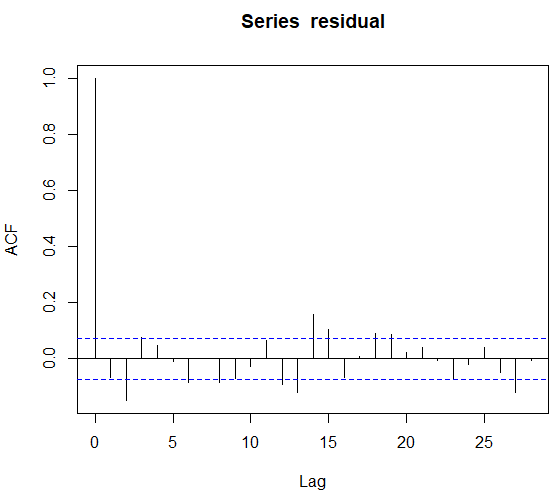
\includegraphics[height=2in]{btcbefno.PNG}
  \caption{ Residual ACF plot for Bitcoin during before period with no penalty}
  \end{subfigure}
% \begin{figure}[h]
  \begin{subfigure}{.49\textwidth}
    \centering
  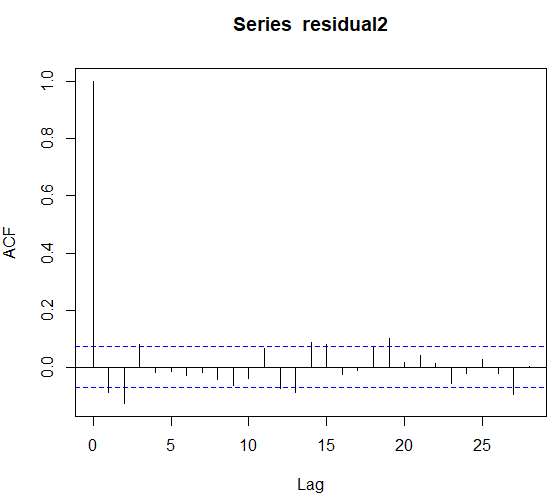
\includegraphics[height=2in]{btcbefstrong.PNG}
  \caption{ Residual ACF plot for Bitcoin during before period with strong penalty}
  \end{subfigure}
  \caption{Residual ACF plot for Bitcoin}
\end{figure}

\begin{figure}[h]
  \begin{subfigure}{.49\textwidth}
    \centering

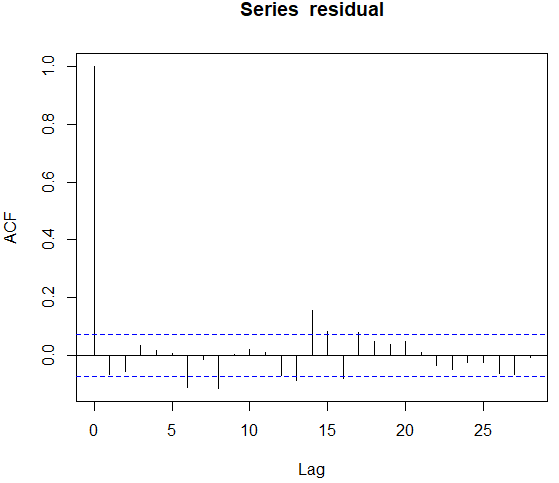
\includegraphics[height=2in]{ethbefno.PNG}
\caption{ Residual ACF plot for Ethereum during before period with no penalty}
  \end{subfigure}
% \begin{figure}[h]
  \begin{subfigure}{.49\textwidth}
  \centering

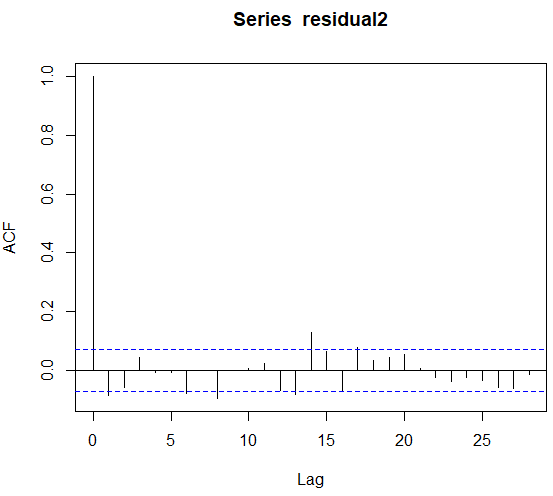
\includegraphics[height=2in]{ethbefstrong.PNG}
\caption{ Residual ACF plot for Ethereum during before period with strong penalty
}
\end{subfigure}
\caption{Residual ACF plot for Ethereum}
\end{figure}




\begin{figure}[h]
  \begin{subfigure}{.49\textwidth}
    \centering
  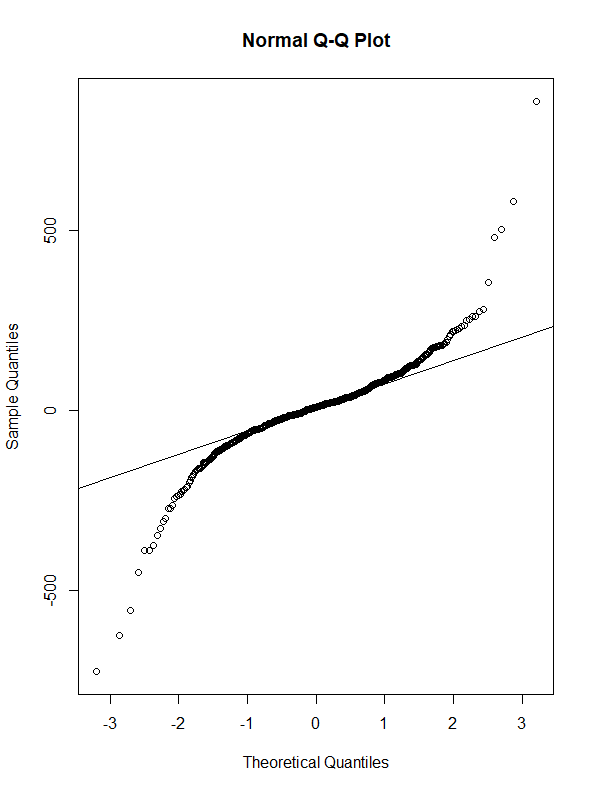
\includegraphics[height=2in]{btcqqbefno.png}
  \caption{ Residual QQ plot for Bitcoin during before period with no penalty}
  \end{subfigure}
% \begin{figure}[h]
  \begin{subfigure}{.49\textwidth}
    \centering
  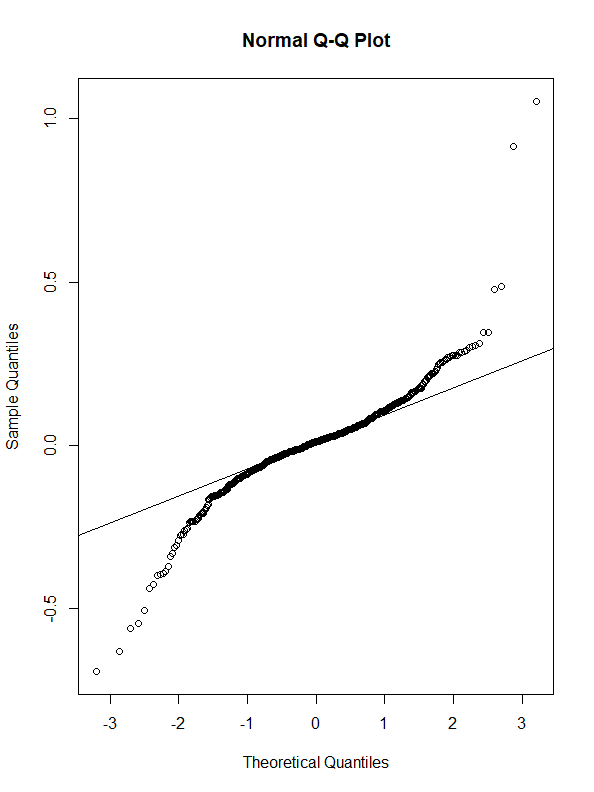
\includegraphics[height=2in]{btcqqbefstrong.png}
  \caption{ Residual QQ plot for Bitcoin during before period with strong penalty}
  \end{subfigure}
  \caption{Residual QQ plot for Bitcoin}
\end{figure}

\begin{figure}[h]
  \begin{subfigure}{.49\textwidth}
    \centering

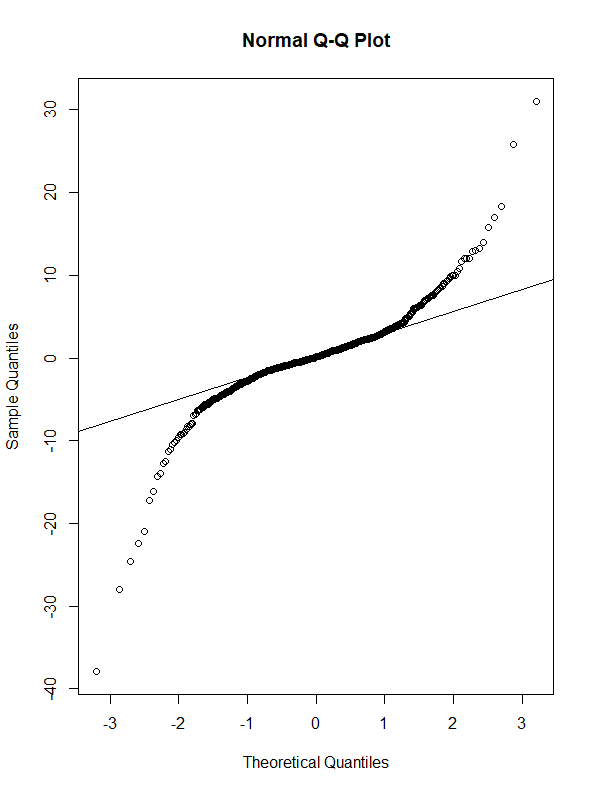
\includegraphics[height=2in]{ethqqbefno.png}
\caption{ Residual QQ plot for Ethereum during before period with no penalty}
  \end{subfigure}
% \begin{figure}[h]
  \begin{subfigure}{.49\textwidth}
  \centering

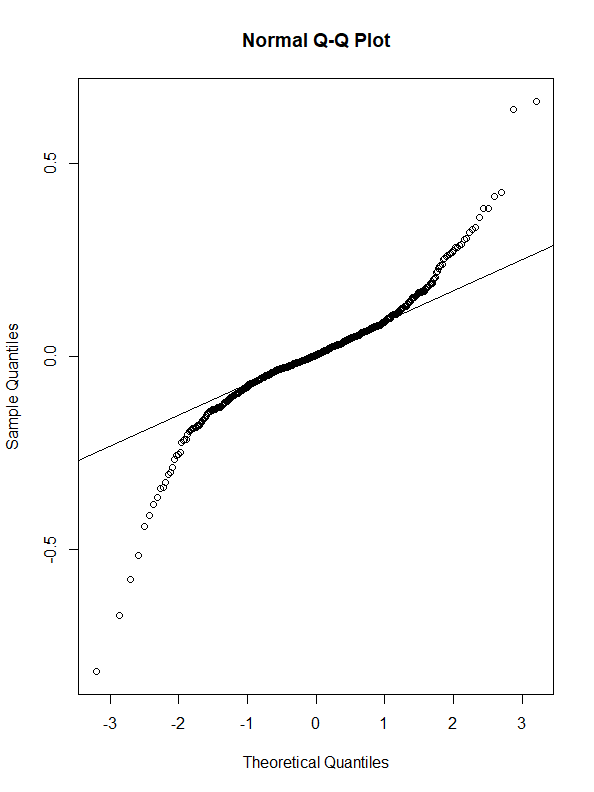
\includegraphics[height=2in]{ethqqbefstrong.png}
\caption{ Residual QQ plot for Ethereum during before period with strong penalty
}
\end{subfigure}
\caption{Residual QQ plot for Ethereum}
\end{figure}

\begin{landscape}
\begin{figure}[h!]
  \caption{Other Parameters}
  \centering
  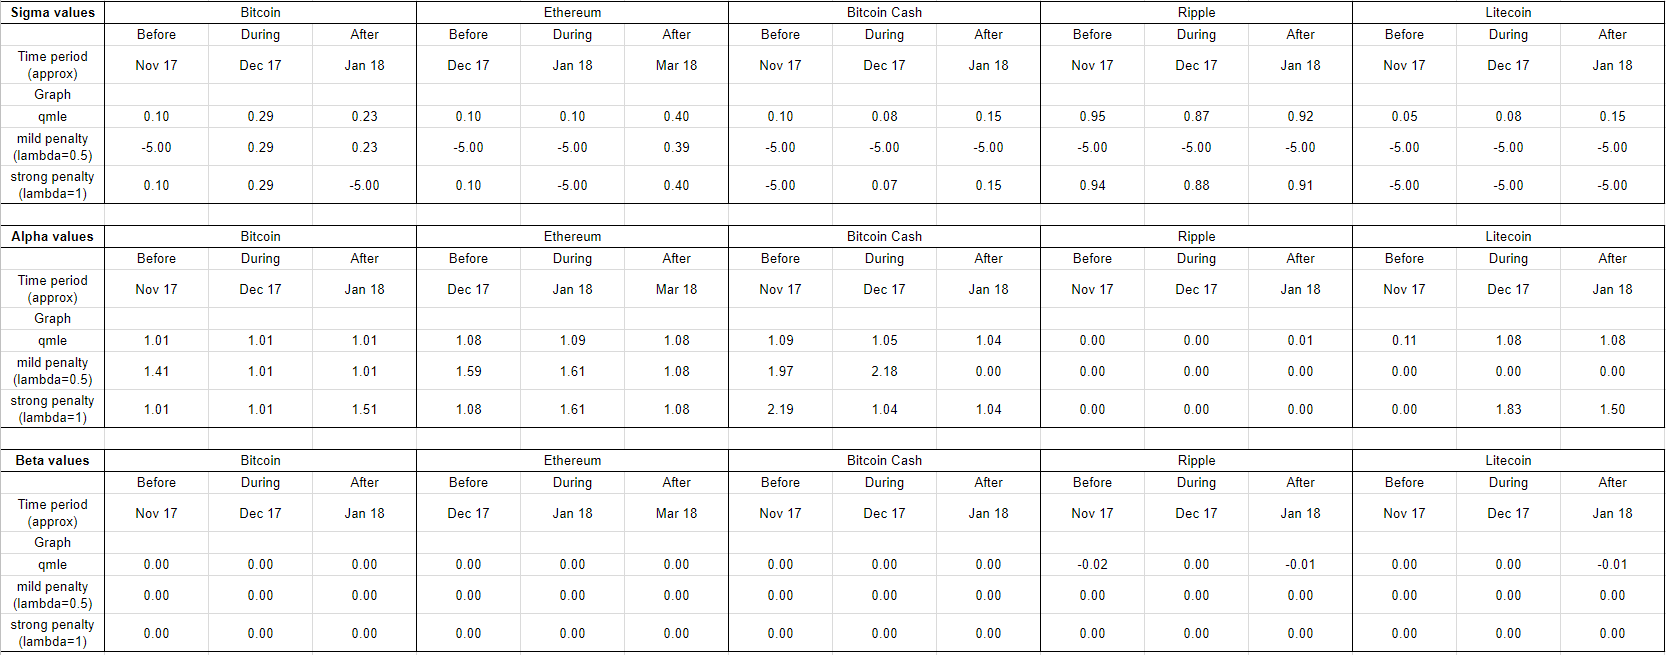
\includegraphics[width=1.4\textwidth]{greeks.PNG}
\end{figure}

\end{landscape}

\end{spacing}
\end{document} to your LaTeX file where you want your
% title page.
%
%%%%%%%%%%%%%%%%%%%%%%%%%%%%%%%%%%%%%%%%%
%\title{Title page with logo}
%----------------------------------------------------------------------------------------
%	PACKAGES AND OTHER DOCUMENT CONFIGURATIONS
%----------------------------------------------------------------------------------------

\documentclass[twocolumns]{IEEEtran} %[xcolor=table]{beamer}%
\usepackage[table]{xcolor}
\usepackage[english]{babel}
\usepackage[utf8x]{inputenc}
\usepackage{amsmath}
\usepackage{graphicx}
\usepackage{setspace}  
\usepackage{lscape}
\usepackage[english]{babel}
\usepackage{subcaption}
% \usepackage{compactenum}
\usepackage[colorinlistoftodos]{todonotes}
% Please add the following required packages to your document preamble:

% If you use beamer only pass "xcolor=table" option, i.e. \documentclass[xcolor=table]{beamer}

\begin{document}

\begin{titlepage}

\newcommand{\HRule}{\rule{\linewidth}{0.5mm}} % Defines a new command for the horizontal lines, change thickness here

\center % Center everything on the page
 
%----------------------------------------------------------------------------------------
%	HEADING SECTIONS
%----------------------------------------------------------------------------------------

\textsc{\LARGE Cornell University}\\[1.5cm] % Name of your university/college
\begin{figure}
  \centering
  
\includegraphics[width=0.25\textwidth]{cornell.png}
\end{figure}

\textsc{\Large ORIE 5640}\\[0.5cm] % Major heading such as course name
\textsc{\large Statistics for Financial Engineering}\\[0.5cm] % Minor heading such as course title

%----------------------------------------------------------------------------------------
%	TITLE SECTION
%----------------------------------------------------------------------------------------

\HRule \\[0.4cm]
{ \huge \bfseries Bubble Detection for Cryptocurrency }\\[0.4cm] % Title of your document
\HRule \\[1.5cm]
 
%----------------------------------------------------------------------------------------
%	AUTHOR SECTION
%----------------------------------------------------------------------------------------

\begin{minipage}{0.4\textwidth}
\begin{flushleft} \large
\emph{Author:}\\
Chen \textsc{Zhong} \\
Chen \textsc{Weijia} \\
Yi \textsc{Shen} \\
Chen \textsc{Peng Yuan} \\

% Your name
\end{flushleft}
\end{minipage}
~
\begin{minipage}{0.4\textwidth}
\begin{flushright} \large
\emph{Professor:} \\
Prof. Edward \textsc{Mehrez} % Supervisor's Name
\end{flushright}
\end{minipage}\\[2cm]

% If you don't want a supervisor, uncomment the two lines below and remove the section above
%\Large \emph{Author:}\\
%John \textsc{Smith}\\[3cm] % Your name

%----------------------------------------------------------------------------------------
%	DATE SECTION
%----------------------------------------------------------------------------------------

{\large May 21, 2018}\\[2cm] % Date, change the \today to a set date if you want to be precise
 
%----------------------------------------------------------------------------------------

\vfill % Fill the rest of the page with whitespace

\end{titlepage}
\onecolumn
\setcounter{tocdepth}{2}
\tableofcontents
\clearpage


\begin{spacing}{1.5}
\begin{abstract}
Since the 2000 dot-com bubble and the 2008-2009 financial crisis, bubbles became an essential issue among the financial industry. Within the past few years, cryptocurrency emerged as a popular asset not only among institutional investors, but also among the retail investors. The problem that we are going to address is to determine in real time whether different cryptocurrencies exhibit a bubble, which has the characteristic of reaching unrealistic price level and then crashes. Our procedure involves Lasso estimation and using the standard stochastic differential equation driven by a Brownian motion to determine whether the process is a strict local martingale. We will illustrate this bubble detection procedure by applying on the cryptocurrency asset class, where we believe price bubbles were widely thought to have existed.
\end{abstract}

\section{Introduction}
Crypotocurrencies became a heated topic recently. Cryptocurrencies had become all over the financial news. In 2008, pseudonymous Satoshi Nakamoto introduced the digital decentralized cryptocurrency, bitcoin. Since then, people have envisioned cryptocurrency as the next generation of currency. Bitcoin has experienced the super-exponential growth. Due to the rise of the popularity of bitcoin, other cryptocurrencies also erupted into the mainstream. This creates a popular demand among all the investors, from institutional investors to retail investors. Cryptocurrencies have become an emerging asset class. At the end of 2017, the price of bitcoin peaked at almost 20,000 USD, and the combined market capitalization of cryptocurrencies reached around 800 billion USD.

Conventional view is that asset bubbles are rare. However, we believe that there are bubbles among the cryptocurrencies. For a bubble to develop among an asset class, first the asset class will start to be in an overheated market in which there are too many buyers who are too keen to buy. As a result, prices rise way too fast, and this situation becomes unsustainable. Eventually, some people realize this and start to sell out of the asset. The whole process goes into reverse equally rapidly, and the bubble bursts. This caused all the people to sell in panic so that prices plunge rapidly. Some of the intuitions behind the finance bubble are when retail investors start to talk about it, the media and news start to cover about the asset class all over the place. However, these are fundamental views without mathematical theory proofs. 

In this paper, we are concentrating on detecting bubbles in cryptocurrencies, including Bitcoin, Bitcoin Cash, Ripples, Litecoin and Ethereum. Our procedure involved using the standard stochastic differential equation driven by a Brownian Motion to determine whether the process is a strict local martingale using QMLE and Lasso estimation.

\section{Bubble Theory}
As shown by Jarrow, Protter and Shimbo\cite{jarrow2011detect}, there are mainly three types of asset price bubbles. Among them, two exist in infinite horizon economies under the weakly complete market which is frictionless, competitive and continuous trading. Hence, we consider the Type Three Bubbles, which exist in finite horizons. According to their theory, a model for asset price process using a  standard stochastic differential equation driven by a Brownian Motion is given as below:
$$dS_t=\sigma(S_t)dW_t+\mu(S_t)dt$$
Under No-arbitrage setting, there exists risk neutral measure under which the SDE satisfies this:
$$S_t=S_0+\int_0^t\sigma(S_s)dW_s$$
whether this type of bubbles exists or not is determined by whether the price process under risk-neutral measure is a strict local martingale. 

\subsection{Theory}
A stochastic process $M = (M_n)_{n\ge n}$ with the relation that $E(M_m|F_n)=M_n$ for any $m\ge n$ is called a martingale.

Here, martingale means a process whose expected future values equals its present value, conditioned on history. The intuition behind the distinction between a martingale and a strict local martingale (in the case where the local martingale $S > 0$) derived from the fact that local martingale is always a supermartingale, which has a decreasing trend in the future expected value. The local martingale is a martingale if and only if it has constant expectation. 

Whether this type of bubbles exists or not is determined by whether the price process under risk-neutral measure is a strict local martingale. More formally, through Comparison Theorem*, we have Type Three Bubbles exist if and only if,
$$\int_{\alpha}^{\infty}\frac{x}{\sigma^2(x)}dx<\infty$$
for all $\alpha>0.$  
\subsection{Intuition}
$$
P_t > E^{Q}  [e^{-r (\tau - t)} P_{\tau} ]
$$
where $P_{\tau}$ is the liquidation value at time $\tau$.

The economic intuition behind this is that the present price is greater than expected future cash flows under the risk neutral measure. According to the fundamental theorem of asset pricing, current price of an asset should be equal to the discounted future cash flow under the risk neutral measure. When price at time t is greater than that value we call it a super martingale. This indicates that the current price of the asset is greater than what the fundamentals of the asset suggests, and that people are not trading on the intrinsic value but on the certain unrealistic expectation, hence the bubble.



\section{Model Selection}
We now consider a proper way to apply the bubble theory to our cryptocurrency data. As implied above in the bubble theory, according to the comparison theorem we need a parametric model for the diffusion term in order to calculate the integral. Hence our objective here is to fit our data to an appropriate parametric model so we can use the parameters derived to perform the bubble test.\\
For the specific methods to fit our data with, we will be considering the following parametric model fitting processes:
\begin{itemize}
\item QMLE (Quasi-Maximum Likelihood Estimator)
\item LASSO (Least Absolute Shrinkage and Selection Operator)
\end{itemize}
\subsection{Base Model}
Consider the following stochastic differential equation;
$$
dX_t = b(\theta_2,X_t)dt+\sigma(\theta_1,X_t)dW_t
$$

This is the most general form of stochastic process to model any kind of price process. Function $b$ is a deterministic function with parameters $\theta_2$ and the  asset price at time $t$, function $\sigma$ is also a deterministic function with parameters $\theta_1$ and asset price. This structure has the flexibility to capture most potential behaviors of cryptocurrencies.

We will determine the precise model to fit our data with later.

\subsection{QMLE}
QMLE stands for Quasi-Maximum Likelihood Estimator, it is a method to estimate parameters of a statistical model very similar to MLE
(Maximum Likelihood Estimator). Both methods choose the parameters that maximize the likelihood function. MLE maximizes the log likelihood function while QMLE maximizes a function that is similar to the log likelihood function but has a simpler version in structure.

The pro of using QMLE is that it specifies a density function that admits specifications of different conditional moments and other distribution characteristics. The con is that it introduces misspecification errors. Hence QMLE requires careful construction of the likelihood function to avoid these errors.

In order to implement QMLE, we need to compare the difference in information presented by the original MLE likelihood and the QMLE approximated likelihood. Here we consider the Kullback-Leibler Information Criterion(KLIC) of $g$ relative to $f$ as: 
$$
 \mathbf{I} (g:f) = \int_{\mathbf{R}} log(\frac{g(\xi)}{f(\xi)})g(\xi)d\xi
$$

KLIC is the rough measure of the closeness between f and g. To approximate $g_t(y_t|x_t)$, we specify a quasi-likelihood function $f_t(y_t|x_t;\theta)$. KLIC of $g_t$ relative to $f_t$ is:
$$
 \mathbf{I} (g_t:f_t;\theta) = \int_{\mathbf{R}} log(\frac{g_t(y_t|x_t)}{f_t(y_t|x_t;\theta)})g_t(y_t|x_t)dy_t
$$

For a sample of T observations we consider the average of T individual KLICs:

$$
 \bar{\mathbf{I}}_T (g_t:f_t;\theta) = \frac{1}{T} \sum_{t=1}^{T}\mathbf{I}(g_t:f_t;\theta)=\frac{1}{T} \sum_{t=1}^{T}(\mathbf{E}[log\,g_t(y_t|x_t)]-\mathbf{E}[log\, f_t(y_t|x_t;\theta)])
$$

We wish to minimize the total KLIC to get a close estimate, hence we need to maximize:

$$
\bar{L}_T(\theta)=\frac{1}{T}\sum_{t = 1}^{T}\mathbf{E}[log\, f_t(y_t|x_t;\theta)]
$$

Since it is not directly observable due to the expectation, in practice, we will try to maximize its sample counterpart:

$$
L_T(y^T,x^T;\theta)=\frac{1}{T}\sum_{t = 1}^{T}log\, f_t(y_t|x_t;\theta)
$$

The resulting $\theta$ will be our quasi-maximum likelihood estimator.

For diffusion process solutions of SDE and observed at discrete times such as our model, we can define the likelihood function using the Markov property. First we can construct the likelihood function $L_n(\theta)$ of the Markovian process X using the conditional distributions:

$$
L_n(\theta) = \prod_{i=1}^{n}p_{\theta}(\Delta_i,X_i|X_{i-1})p_{\theta}(X_0)
$$

Assuming $p_{\theta}(X_0)=1$ and take log to the likelihood function we get a log-likelihood function:

$$
l_n(\theta)=log\,L_n(\theta)=\sum_{i=1}^n l_i(\theta)+log(p_{\theta}(X_0))=\sum_{i=1}^n log\,p_{\theta}(\Delta_i,X_i |X_{i-1})
$$

Since exact likelihood inference is not always possible, explicit form of the function is rarely known. For parameters in the diffusion coefficient, MLE rate of convergence if order $\sqrt{n}$ while the estimators for the drift convergence is of order $\sqrt{T}$. Hence we require $n\Delta=T \to \infty$. Using the Euler-Maruyama discretization scheme as introduced by the work of Genon-Catalot and Jacod(1993) we get our approximated negative log likelihood function:

$$
l_n(X_n,\theta) = -\frac{1}{2}\sum_{i=1}^{n}\{ log \,\textbf{det}(\sigma_{i-1}(\theta_1)) + \frac{1}{\Delta_n}\Sigma_{i-1}^{-1}(\theta_1)[\Delta X_i-\Delta_n b_{i-1}(\theta_2)]^{\otimes 2} \}
$$

Where $\theta=(\theta_1,\theta_2),\, \Delta X_i = X_{t_i}-X_{t_{i-1}},\, \Sigma_i(\theta_1) = \Sigma(\theta_1,X_t),\, b_i(\theta_2)=b(\theta_2,X_{t_i}),\, \Sigma=\sigma^{\otimes 2},\, A^{\otimes 2}=A^TA$, and $A^{-1}$ the inverse of A, then the QML estimator of $\theta$ is:

$$
\tilde{\theta}_n = arg\min_{\theta}\, l_n(X_n,\theta)
$$

Notice here that the sign for the likelihood function is negative, which turns the argmin function to maximization. The approximate log-likelihood function consists of 2 parts: stochastic volatility term, and the standardized price change term. This approximate function has the characteristics of log likelihood and certainly components of other model specifications as well.

In our case, we will be using the built-in solver from the Yuima package which uses the contrast function from the work of Genon-Catalot and Jacod \cite{genon1993estimation}.

\subsection{LASSO}
On top of QMLE, we will also be applying LASSO (least absolute shrinkage and selection operator) as an improvement to the parameter selection process. It is a regression analysis method that performs both variable selection and regularization. LASSO can enhance prediction accuracy and interpretability by streamlining the selection of variables and highlight the more significant ones. It does so by putting constraints on parameters, and introduces regularizers, the argmin function will try to minimize the number and size of coefficients while maintaining the efficiency of the results.

Using LASSO is very useful for models with many parameters since it can eliminate unnecessary coefficients. It is also useful in our implementation since we aim at modeling with a general model, with too many parameters, we might risk over fitting our data. Hence LASSO is very useful for modeling in our case to eliminate unnecessary parameters, even when there are only a few we still want to choose the most significant ones.

QMLE + LASSO parameter selection function:

$$
\min l_n(X_n,\theta)+ \sum^p_{j=1}\lambda_{n,j} |\theta_{2j}| + \sum^q_{k = 1}\gamma_{n,k} |\theta_{1k}|
$$

The minimization problem (maximization for the log likelihood) here aims at finding the parameters that maximizes the QMLE function while keeping the LASSO terms minimum. 

Depending on the sensitivity towards the size of parameter, we will have 3 different degrees of penalty settings as a parameter on LASSO:
\begin{itemize}
\item No penalty: no LASSO term in the function, only the QMLE term
\item Mild penalty: small penalty on magnitude of parameters, decrease the occurrence of large parameters, prevents collinearity of variables
\item Strong penalty: big penalty on magnitude of parameters, eliminate the occurrence of large parameters
\end{itemize}

\subsection{CKLS Model}
Since we don't know the exact property of cryptocurrency price changes, the best approximation is to treat them like asset price. Our simplest model for stock price is geometric brownian motion (GBM), and a good model for short term interest rate is the Vasicek short rate model, and there are a lot more to choose from. We want something that has enough flexibility to describe a variety of characteristic to allow for generality.

Chan, Karolyi, Longstaff and Sanders (CKLS) achieves just that:
$$
dX_t = (\alpha + \beta X_t)dt + \sigma X_t^{\gamma}dW_t
$$

By modifying the parameters, it can become Merton model, Vasicek model, Cox model, GBM model and many more. It has the flexibility to describe the behavior of cryptocurrency.

More importantly, the diffusion term is a power function: $\sigma X_t^{\gamma}$, whose $\gamma$ parameter is the indicator for the bubble test
\subsection{Bubble Test}
As mentioned in the bubble theory, we want to test whether $\int^{\infty}_{\alpha}\frac{x}{\sigma^2(x)}dx < \infty$.

Substitute $\sigma (x)$ with $\sigma x^{\gamma}$:

\begin{equation}
\begin{aligned}
\int^{\infty}_{\alpha}\frac{x}{\sigma^2(x)}dx &= \int^{\infty}_{\alpha}\frac{x}{(\sigma x^{\gamma})^2}dx \\
&= \frac{1}{\sigma^2}\int^{\infty}_{\alpha}\frac{x}{x^{2\gamma}}dx \\
&= \frac{1}{\sigma^2}\int^{\infty}_{\alpha}x^{1-2\gamma}dx \\
&= \frac{1}{\sigma^2}\frac{1}{2-2\gamma}x^{2-2\gamma} |_{\alpha}^{\infty}
\end{aligned}
\end{equation}

Integral goes to infinity if and only if $\gamma > 1$, hence according to comparison theorem, the process X is:
\begin{itemize}
\item a strict local martingale if $\gamma > 1$ (bubble)
\item a martingale if $\gamma \le 1$ (not bubble)
\end{itemize}

\section{Evaluation}

We evaluated the model based on five major cryptocurrencies during three manually selected periods: before the bubble appears (when the price soars), during the bubble happens (when the price remain high), and after the bubble bursts (when the price plummets). We expect to see that our model output that there is a bubble during the first period, and not a bubble after the second period. 

For each period, we used plain QMLE method, QMLE with mild LASSO regularization and QMLE with strong LASSO regularization to evaluate the $\gamma$ parameters. 

At the end of this paper is a table of results we generated using the YUIMA package \cite{brouste2013parameter}. 

From the result (as shown in table I) along with our other observations, we come up with the following findings:

\subsection{Effect of model}
\begin{enumerate}
\item All the estimation methods generate expected results ($\gamma>1$) for ``before the bubble'' period for all the cryptocurrencies. 
\item For estimations of ``during the bubble'' periods, we are more likely to have $\gamma>1$ when a sudden spike of price is included in that period.
\item Our estimation for gamma in ``during the bubble'' and ``after the bubble'' periods vary, while the plain QMLE methods generates desirable results.  
\end{enumerate}

\subsection{Robustness of estimator}
Significant ourliers in the table can be observed in the evaluation for Ripple, where the estimated $\gamma$ are around zero for before and after the bubble periods. A significant difference between ripple and other cryptocurrencies is that its price is considerably low ($<$\$5) throughout the whole period, compared with some thousand dollars of value for cryptos like bitcoin and bitcoin cash. Therefore, we suspect that the value of the price could influence the performance of our model. We therefore added a big constant (1000) to the Ripple prices and evaluated it using the model and the $\gamma$ we got then all exceed 1. Though a rough method, it somehow indicates that the stability of such a model might be a concern and preprocessing the data using some normalization technique might be helpful.

\subsection{Effect of LASSO regularizer}

It is quite surprise to the author that the estimated values generated by adding the LASSO regularizer to the plain QMLE method is quite large. This not only true for the $\gamma$ value, but also for total sum of absolute value of $\alpha, \beta, \gamma$ and $\sigma$ in the model, which goes against our motive for adding such a regularizer. Intuitively, LASSO regularizer applies to a model with many (perhaps hundreds or thousands of) parameters where we wish to have most of the parameters close to zero and a few comparatively large values. The CKLS model only have 4 parameters --- $\alpha, \beta, \gamma$ and $\sigma$, all of which contain significant information of the model. The author thus doubts the effect of applying the LASSO regularizer to such a model, given the unexpected results.

\subsection{Higher frequency data}

We also implemented the evaluation for higher frequency data (minute data for 1-2 weeks) but got some quite disappointing results. All the estimators render $\gamma\geq1$ for all periods and all cryptocurrencies. We doubt that such a model might be prone to noises in high frequency data and thus decide not to reveal the results.  

\subsection{Robustness: Window Extension}
In previous results, we set our time window separately for the before, during and after periods. We wonder if our test will yield more interesting result if we run our test with cumulative data. As shown in table II, we ran our test using cumulative data in the before period and the before and during period.

We are most interested in the before and during period. When we run our test with cumulative data, all parameters except for that of Ripple's are greater than 1, meaning all asset show sign of bubble when we run the cumulative data up to when the suspected bubble burst.

\subsection{Specification Test}
In order to test whether CKLS model is indeed a good fit for the cryptocurrency market, we need to check the standardized residual:
$$
\epsilon_t = \frac{\Delta S_t-\hat{b}(\alpha,\beta,S_{t-1})\Delta_t}{\hat{\sigma}(\sigma,S_{t-1})}
$$

If our model is a good fit then: $\epsilon_t \approx \Delta W_t \sim N(0,\Delta_t)$.
\subsubsection{ACF-plot}
The residuals from our model should be stationary series. From ACF plots of residuals (Fig.1-2) we can see that there are no significant spikes, meaning the residuals are stationary and that the resulting model is a decent fit for our data, and any potential issue of the model might stem from the implementation procedure.
\subsubsection{QQ-plot}
As shown in the QQ-plot (Fig.3-4), the standardized residuals are not exactly normally distributed, but all of them have heavier tails than the normal distribution. The deviation from the normal are very much even on both ends, meaning the distribution is not skewed to one side. This is an evidence that standard Brownian Motion may not be the fundamental drive of the bubble price process. As an indication for future work, this means that instead of modeling using normal distribution, we can assume that the distribution is t-distribution and base our model on t-distribution, which can adjust for the heavier tail. 
\section{Conclusion}
In this project, we studied the bubble theory \cite{jarrow2011detect} proposed by Jarrow, Kchia, and Protter and analyzed the mathematics behind such theory, We selected CKLS stochastic model for evaluation and implemented it on 5 major cryptocurrencies prices at the end of 2017 when we witness significantly soaring prices. The quasi-maximum likelihood estimator generates remarkable results for bubble detection while the effect of LASSO regularizer is less desirable.

\bibliographystyle{unsrt}
\bibliography{ref}

\begin{landscape}
\begin{table}[]
\centering
\resizebox{\textwidth}{!}{%
\begin{tabular}{|c|ccc|ccc|ccc|ccc|ccc|}
\hline
Gamma values & \multicolumn{3}{c|}{Bitcoin} & \multicolumn{3}{c|}{Ethereum} & \multicolumn{3}{c|}{Bitcoin Cash} & \multicolumn{3}{c|}{Ripple} & \multicolumn{3}{c|}{Litecoin} \\ \hline
 & \multicolumn{1}{c|}{Before} & \multicolumn{1}{c|}{During} & After & \multicolumn{1}{c|}{Before} & \multicolumn{1}{c|}{During} & After & \multicolumn{1}{c|}{Before} & \multicolumn{1}{c|}{During} & After & \multicolumn{1}{c|}{Before} & \multicolumn{1}{c|}{During} & After & \multicolumn{1}{c|}{Before} & \multicolumn{1}{c|}{During} & After \\ \hline
Time period (approx) & \multicolumn{1}{c|}{Nov 17} & \multicolumn{1}{c|}{Dec 17} & Jan 18 & \multicolumn{1}{c|}{Dec 17} & \multicolumn{1}{c|}{Jan 18} & Mar 18 & \multicolumn{1}{c|}{Nov 17} & \multicolumn{1}{c|}{Dec 17} & Jan 18 & \multicolumn{1}{c|}{Nov 17} & \multicolumn{1}{c|}{Dec 17} & Jan 18 & \multicolumn{1}{c|}{Nov 17} & \multicolumn{1}{c|}{Dec 17} & Jan 18 \\ \hline
qmle & 1.000 & 0.890 & 0.910 & 1.000 & 0.806 & 0.797 & 1.010 & 1.040 & 0.950 & -0.010 & -0.135 & -0.087 & 1.120 & 1.030 & 0.920 \\ \cline{1-1}
\rowcolor[HTML]{C0C0C0} 
std.qmle & 0.021 & 0.013 & 0.016 & 0.021 & 0.017 & 0.008 & 0.011 & 0.011 & 0.016 & 9.211 & 0.420 & 6.490 & 0.035 & 0.017 & 0.023 \\ \cline{1-1}
mild penalty ($\lambda$=0.5) & 6.655 & 0.890 & 0.910 & 8.000 & 0.806 & 2.937 & 8.000 & 8.000 & 5.526 & 0.000 & 4.677 & 0.000 & 8.000 & 8.000 & 7.630 \\ \cline{1-1}
\rowcolor[HTML]{C0C0C0} 
std.qmle & 0.015 & 0.009 & 0.011 & 0.015 & 0.012 & 0.006 & 0.008 & 0.008 & 0.011 & 0.003 & 0.297 & 0.005 & 0.025 & 0.012 & 0.016 \\ \cline{1-1}
strong penalty ($\lambda$=1) & 1.000 & 0.890 & 3.300 & 8.000 & 0.806 & 0.795 & 8.000 & 1.040 & 0.949 & 0.000 & 0.476 & 0.000 & 8.000 & 8.000 & 7.630 \\ \cline{1-1}
\rowcolor[HTML]{C0C0C0} 
std.qmle & 0.015 & 0.009 & 0.011 & 0.015 & 0.012 & 0.006 & 0.008 & 0.008 & 0.011 & 0.001 & 0.297 & 0.003 & 0.025 & 0.012 & 0.016 \\ \hline
\end{tabular}
}
\caption{Estimated $\gamma$ and its standard deviation for different cryptocurrencies in different periods. ($\lambda$ $\text{ indicates the shrinkage level.}$)}

\label{result}
\end{table}

\begin{table}[]
\centering

\resizebox{\textwidth}{!}{%
\begin{tabular}{|c|cc|cc|cc|cc|cc|}
\hline
Gamma values              & \multicolumn{2}{c|}{Bitcoin}         & \multicolumn{2}{c|}{Ethereum}        & \multicolumn{2}{c|}{Bitcoin Cash}    & \multicolumn{2}{c|}{Ripple}          & \multicolumn{2}{c|}{Litecoin}        \\ \hline
& \multicolumn{1}{c|}{Before} & Before \& During & \multicolumn{1}{c|}{Before} & Before \& During & \multicolumn{1}{c|}{Before} & Before \& During
& \multicolumn{1}{c|}{Before} & Before \& During & \multicolumn{1}{c|}{Before} & Before \& During\\ \hline
Time period (approx)      
& \multicolumn{1}{c|}{Nov 17} & Nov-Dec 17 & \multicolumn{1}{c|}{Dec 17} & Dec 17-Jan 18 & \multicolumn{1}{c|}{Nov 17} & Nov-Dec 17& \multicolumn{1}{c|}{Nov 17} & Nov-Dec 17 & \multicolumn{1}{c|}{Nov 17} & Nov-Dec 17 \\ \hline
qmle   & 1.000    & 1.001  & 1.000    & 1.028& 1.011    & 1.009  & -0.010   & -0.067 & 1.130    & 1.103  \\ \cline{1-1}
\rowcolor[HTML]{C0C0C0} 
std.qmle   & 0.021    & 0.021  & 0.035    & 0.018  & 0.011    & 0.008  & 9.211    & 1.045  & 0.035    & 0.015  \\ \cline{1-1}
mild penalty ($\lambda$=0.5) & 6.655    & 8.000  & 8.000    & 8.000  & 8.000    & 7.922  & 0.000   & 0.000  & 8.000    & 8.000  \\ \cline{1-1}
\rowcolor[HTML]{C0C0C0} 
std.qmle  & 0.015    & 0.015  & 0.025    & 0.013  & 0.008    & 0.005  & 0.003    & 0.005  & 0.025    & 0.011  \\ \cline{1-1}
strong penalty ($\lambda$=1) & 1.000    & 8.000  & 0.997    & 8.000  & 8.000    & 1.008  & 0.000    & -0.065  & 8.000    & 8.000  \\ \cline{1-1}
\rowcolor[HTML]{C0C0C0} 
std.qmle  & 0.015    & 0.015  & 0.025    & 0.013  & 0.008    & 0.005  & 0.001    & 0.739  & 0.025    & 0.011  \\ \hline
\end{tabular}%
}
\label{my-label}
\caption{Estimated $\gamma$ and its standard deviation for different cryptocurrencies in before and before/during periods. ($\lambda$ $\text{ indicates the shrinkage level.}$)}
\end{table}
% \begin{table}[]
% \centering
% \begin{tabular}{|c|ccc|ccc|ccc|ccc|ccc|}
% \hline
% Gamma values & \multicolumn{3}{c|}{Bitcoin} & \multicolumn{3}{c|}{Ethereum} & \multicolumn{3}{c|}{Bitcoin Cash} & \multicolumn{3}{c|}{Ripple} & \multicolumn{3}{c|}{Litecoin} \\ \hline
%  & \multicolumn{1}{c|}{Before} & \multicolumn{1}{c|}{During} & After & \multicolumn{1}{c|}{Before} & \multicolumn{1}{c|}{During} & After & \multicolumn{1}{c|}{Before} & \multicolumn{1}{c|}{During} & After & \multicolumn{1}{c|}{Before} & \multicolumn{1}{c|}{During} & After & \multicolumn{1}{c|}{Before} & \multicolumn{1}{c|}{During} & After \\ \hline
% Time period (approx) & \multicolumn{1}{c|}{Nov} & \multicolumn{1}{c|}{Nov-Dec} & Nov-Jan & \multicolumn{1}{c|}{Nov} & \multicolumn{1}{c|}{Nov-Dec} & Nov-Jan & \multicolumn{1}{c|}{Nov} & \multicolumn{1}{c|}{Nov-Dec} & Nov-Jan & \multicolumn{1}{c|}{Nov} & \multicolumn{1}{c|}{Nov-Dec} & Nov-Jan & \multicolumn{1}{c|}{Nov} & \multicolumn{1}{c|}{Nov-Dec} & Nov-Jan \\ \hline
% qmle 
% & 1.000 & 1.001 & 1.001 & 0.999 & 1.028 & 1.022 & 1.011 & 1.009 & 0.987 & -0.019 & -0.067 & -0.084 & 1.130 & 1.103 & 1.090 \\ \cline{1-1}
% \rowcolor[HTML]{C0C0C0} 
% std.qmle 
% & 0.021 & 0.011 & 0.009 & 0.035 & 0.018 & 0.013 & 0.011 & 0.008 & 0.007 & 4.835 & 1.045 & 0.429 & 0.035 & 0.015 & 0.013 \\ \cline{1-1}
% mild penalty ($\lambda$=0.5) 
% & 6.655 & 6.385 & 6.391 & 8.000 & 8.000 & 8.000 & 8.000 & 7.922 & 0.986 & -4.944 & 0.000 & 8.000 & 8.000 & 8.000 & 8.000 \\ \cline{1-1}
% \rowcolor[HTML]{C0C0C0} 
% std.qmle 
% & 0.015 & 0.008 & 0.007 & 0.025 & 0.013 & 0.009 & 0.008 & 0.005 & 0.005 & 0.004 & 0.005 & 0.303 & 0.025 & 0.011 & 0.009 \\ \cline{1-1}
% strong penalty ($\lambda$=1)
% & 1.000 & 1.000 & 1.000 & 0.997 & 8.000 & 8.000 & 8.000 & 1.001 & 6.945 & 2.437 & -0.065 & 0.070 & 8.000 & 8.000 & 8.000 \\ \cline{1-1}
% \rowcolor[HTML]{C0C0C0} 
% std.qmle 
% & 0.015 & 0.008 & 0.007 & 0.025 & 0.013 & 0.009 & 0.008 & 0.005 & 0.005 & 0.001 & 0.739 & 0.303 & 0.025 & 0.011 & 0.009 \\ \hline
% \end{tabular}
% \caption{Estimated $\gamma$ and its standard deviation for different cryptocurrencies in different periods.(cumulative) ($\lambda$ $\text{ indicates the shrinkage level.}$)}

% \label{result}
% \end{table}
\end{landscape}

\begin{figure}[h]
  \begin{subfigure}{.49\textwidth}
    \centering
  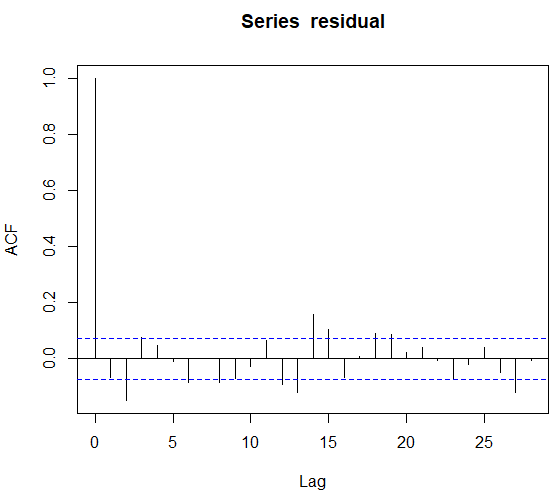
\includegraphics[height=2in]{btcbefno.PNG}
  \caption{ Residual ACF plot for Bitcoin during before period with no penalty}
  \end{subfigure}
% \begin{figure}[h]
  \begin{subfigure}{.49\textwidth}
    \centering
  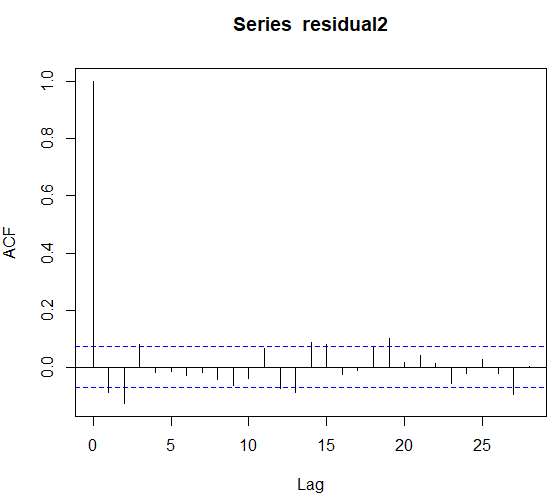
\includegraphics[height=2in]{btcbefstrong.PNG}
  \caption{ Residual ACF plot for Bitcoin during before period with strong penalty}
  \end{subfigure}
  \caption{Residual ACF plot for Bitcoin}
\end{figure}

\begin{figure}[h]
  \begin{subfigure}{.49\textwidth}
    \centering

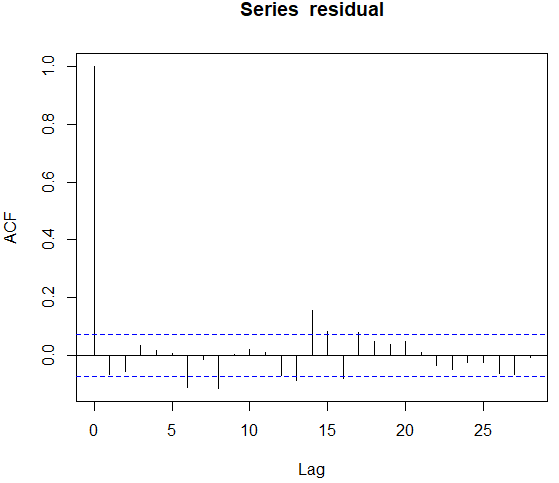
\includegraphics[height=2in]{ethbefno.PNG}
\caption{ Residual ACF plot for Ethereum during before period with no penalty}
  \end{subfigure}
% \begin{figure}[h]
  \begin{subfigure}{.49\textwidth}
  \centering

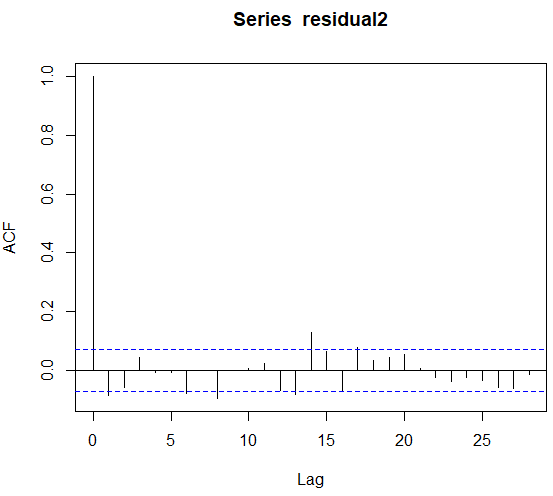
\includegraphics[height=2in]{ethbefstrong.PNG}
\caption{ Residual ACF plot for Ethereum during before period with strong penalty
}
\end{subfigure}
\caption{Residual ACF plot for Ethereum}
\end{figure}




\begin{figure}[h]
  \begin{subfigure}{.49\textwidth}
    \centering
  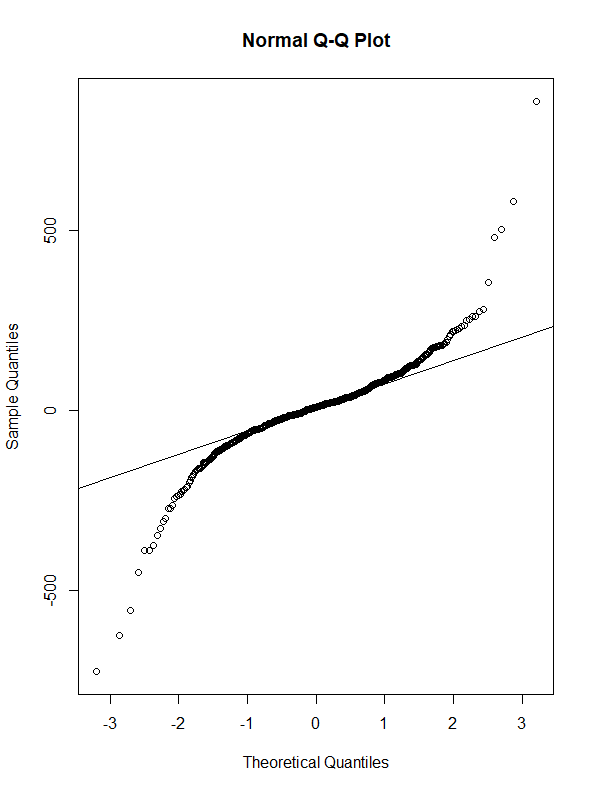
\includegraphics[height=2in]{btcqqbefno.png}
  \caption{ Residual QQ plot for Bitcoin during before period with no penalty}
  \end{subfigure}
% \begin{figure}[h]
  \begin{subfigure}{.49\textwidth}
    \centering
  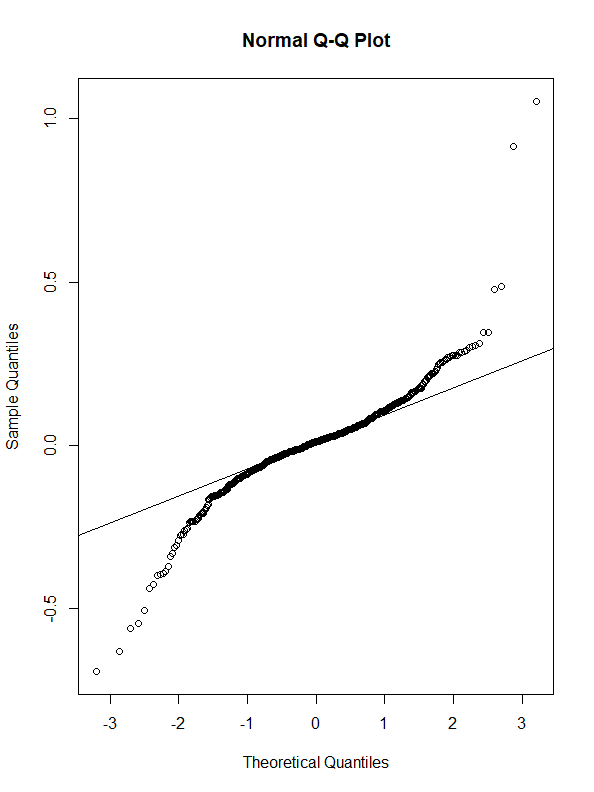
\includegraphics[height=2in]{btcqqbefstrong.png}
  \caption{ Residual QQ plot for Bitcoin during before period with strong penalty}
  \end{subfigure}
  \caption{Residual QQ plot for Bitcoin}
\end{figure}

\begin{figure}[h]
  \begin{subfigure}{.49\textwidth}
    \centering

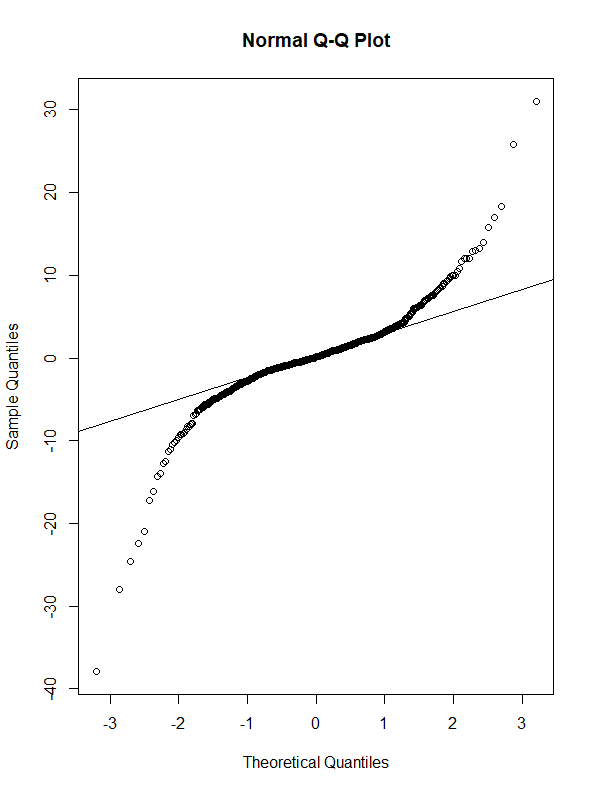
\includegraphics[height=2in]{ethqqbefno.png}
\caption{ Residual QQ plot for Ethereum during before period with no penalty}
  \end{subfigure}
% \begin{figure}[h]
  \begin{subfigure}{.49\textwidth}
  \centering

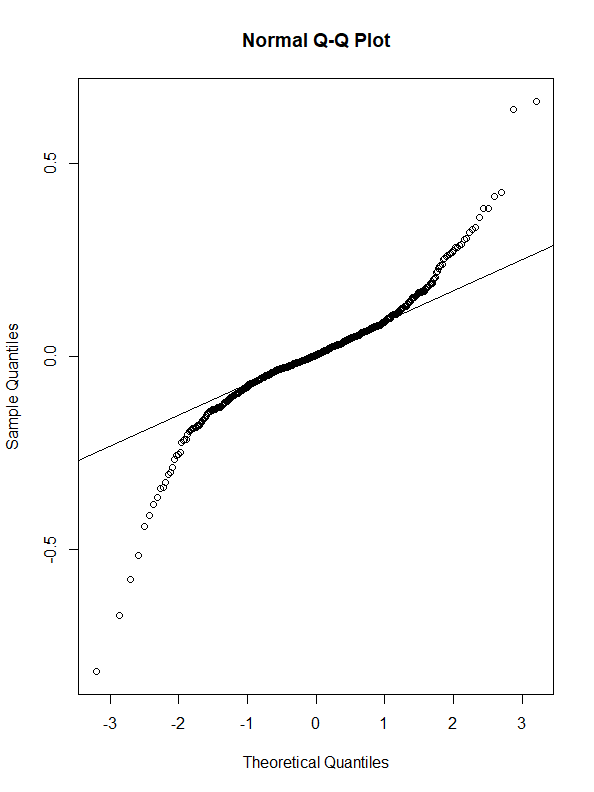
\includegraphics[height=2in]{ethqqbefstrong.png}
\caption{ Residual QQ plot for Ethereum during before period with strong penalty
}
\end{subfigure}
\caption{Residual QQ plot for Ethereum}
\end{figure}

\begin{landscape}
\begin{figure}[h!]
  \caption{Other Parameters}
  \centering
  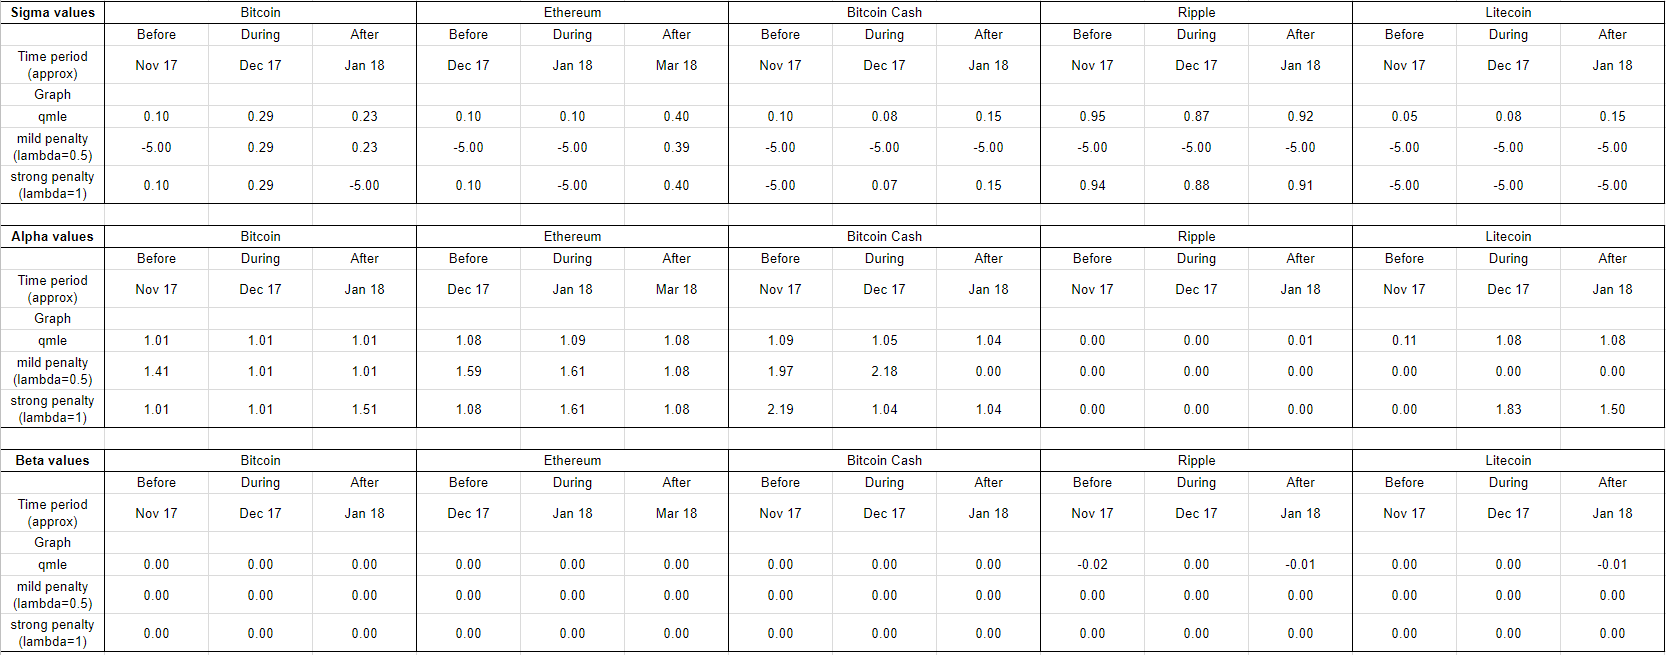
\includegraphics[width=1.4\textwidth]{greeks.PNG}
\end{figure}

\end{landscape}

\end{spacing}
\end{document} to your LaTeX file where you want your
% title page.
%
%%%%%%%%%%%%%%%%%%%%%%%%%%%%%%%%%%%%%%%%%
%\title{Title page with logo}
%----------------------------------------------------------------------------------------
%	PACKAGES AND OTHER DOCUMENT CONFIGURATIONS
%----------------------------------------------------------------------------------------

\documentclass[twocolumns]{IEEEtran} %[xcolor=table]{beamer}%
\usepackage[table]{xcolor}
\usepackage[english]{babel}
\usepackage[utf8x]{inputenc}
\usepackage{amsmath}
\usepackage{graphicx}
\usepackage{setspace}  
\usepackage{lscape}
\usepackage[english]{babel}
\usepackage{subcaption}
% \usepackage{compactenum}
\usepackage[colorinlistoftodos]{todonotes}
% Please add the following required packages to your document preamble:

% If you use beamer only pass "xcolor=table" option, i.e. \documentclass[xcolor=table]{beamer}

\begin{document}

\begin{titlepage}

\newcommand{\HRule}{\rule{\linewidth}{0.5mm}} % Defines a new command for the horizontal lines, change thickness here

\center % Center everything on the page
 
%----------------------------------------------------------------------------------------
%	HEADING SECTIONS
%----------------------------------------------------------------------------------------

\textsc{\LARGE Cornell University}\\[1.5cm] % Name of your university/college
\begin{figure}
  \centering
  
\includegraphics[width=0.25\textwidth]{cornell.png}
\end{figure}

\textsc{\Large ORIE 5640}\\[0.5cm] % Major heading such as course name
\textsc{\large Statistics for Financial Engineering}\\[0.5cm] % Minor heading such as course title

%----------------------------------------------------------------------------------------
%	TITLE SECTION
%----------------------------------------------------------------------------------------

\HRule \\[0.4cm]
{ \huge \bfseries Bubble Detection for Cryptocurrency }\\[0.4cm] % Title of your document
\HRule \\[1.5cm]
 
%----------------------------------------------------------------------------------------
%	AUTHOR SECTION
%----------------------------------------------------------------------------------------

\begin{minipage}{0.4\textwidth}
\begin{flushleft} \large
\emph{Author:}\\
Chen \textsc{Zhong} \\
Chen \textsc{Weijia} \\
Yi \textsc{Shen} \\
Chen \textsc{Peng Yuan} \\

% Your name
\end{flushleft}
\end{minipage}
~
\begin{minipage}{0.4\textwidth}
\begin{flushright} \large
\emph{Professor:} \\
Prof. Edward \textsc{Mehrez} % Supervisor's Name
\end{flushright}
\end{minipage}\\[2cm]

% If you don't want a supervisor, uncomment the two lines below and remove the section above
%\Large \emph{Author:}\\
%John \textsc{Smith}\\[3cm] % Your name

%----------------------------------------------------------------------------------------
%	DATE SECTION
%----------------------------------------------------------------------------------------

{\large May 21, 2018}\\[2cm] % Date, change the \today to a set date if you want to be precise
 
%----------------------------------------------------------------------------------------

\vfill % Fill the rest of the page with whitespace

\end{titlepage}
\onecolumn
\setcounter{tocdepth}{2}
\tableofcontents
\clearpage


\begin{spacing}{1.5}
\begin{abstract}
Since the 2000 dot-com bubble and the 2008-2009 financial crisis, bubbles became an essential issue among the financial industry. Within the past few years, cryptocurrency emerged as a popular asset not only among institutional investors, but also among the retail investors. The problem that we are going to address is to determine in real time whether different cryptocurrencies exhibit a bubble, which has the characteristic of reaching unrealistic price level and then crashes. Our procedure involves Lasso estimation and using the standard stochastic differential equation driven by a Brownian motion to determine whether the process is a strict local martingale. We will illustrate this bubble detection procedure by applying on the cryptocurrency asset class, where we believe price bubbles were widely thought to have existed.
\end{abstract}

\section{Introduction}
Crypotocurrencies became a heated topic recently. Cryptocurrencies had become all over the financial news. In 2008, pseudonymous Satoshi Nakamoto introduced the digital decentralized cryptocurrency, bitcoin. Since then, people have envisioned cryptocurrency as the next generation of currency. Bitcoin has experienced the super-exponential growth. Due to the rise of the popularity of bitcoin, other cryptocurrencies also erupted into the mainstream. This creates a popular demand among all the investors, from institutional investors to retail investors. Cryptocurrencies have become an emerging asset class. At the end of 2017, the price of bitcoin peaked at almost 20,000 USD, and the combined market capitalization of cryptocurrencies reached around 800 billion USD.

Conventional view is that asset bubbles are rare. However, we believe that there are bubbles among the cryptocurrencies. For a bubble to develop among an asset class, first the asset class will start to be in an overheated market in which there are too many buyers who are too keen to buy. As a result, prices rise way too fast, and this situation becomes unsustainable. Eventually, some people realize this and start to sell out of the asset. The whole process goes into reverse equally rapidly, and the bubble bursts. This caused all the people to sell in panic so that prices plunge rapidly. Some of the intuitions behind the finance bubble are when retail investors start to talk about it, the media and news start to cover about the asset class all over the place. However, these are fundamental views without mathematical theory proofs. 

In this paper, we are concentrating on detecting bubbles in cryptocurrencies, including Bitcoin, Bitcoin Cash, Ripples, Litecoin and Ethereum. Our procedure involved using the standard stochastic differential equation driven by a Brownian Motion to determine whether the process is a strict local martingale using QMLE and Lasso estimation.

\section{Bubble Theory}
As shown by Jarrow, Protter and Shimbo\cite{jarrow2011detect}, there are mainly three types of asset price bubbles. Among them, two exist in infinite horizon economies under the weakly complete market which is frictionless, competitive and continuous trading. Hence, we consider the Type Three Bubbles, which exist in finite horizons. According to their theory, a model for asset price process using a  standard stochastic differential equation driven by a Brownian Motion is given as below:
$$dS_t=\sigma(S_t)dW_t+\mu(S_t)dt$$
Under No-arbitrage setting, there exists risk neutral measure under which the SDE satisfies this:
$$S_t=S_0+\int_0^t\sigma(S_s)dW_s$$
whether this type of bubbles exists or not is determined by whether the price process under risk-neutral measure is a strict local martingale. 

\subsection{Theory}
A stochastic process $M = (M_n)_{n\ge n}$ with the relation that $E(M_m|F_n)=M_n$ for any $m\ge n$ is called a martingale.

Here, martingale means a process whose expected future values equals its present value, conditioned on history. The intuition behind the distinction between a martingale and a strict local martingale (in the case where the local martingale $S > 0$) derived from the fact that local martingale is always a supermartingale, which has a decreasing trend in the future expected value. The local martingale is a martingale if and only if it has constant expectation. 

Whether this type of bubbles exists or not is determined by whether the price process under risk-neutral measure is a strict local martingale. More formally, through Comparison Theorem*, we have Type Three Bubbles exist if and only if,
$$\int_{\alpha}^{\infty}\frac{x}{\sigma^2(x)}dx<\infty$$
for all $\alpha>0.$  
\subsection{Intuition}
$$
P_t > E^{Q}  [e^{-r (\tau - t)} P_{\tau} ]
$$
where $P_{\tau}$ is the liquidation value at time $\tau$.

The economic intuition behind this is that the present price is greater than expected future cash flows under the risk neutral measure. According to the fundamental theorem of asset pricing, current price of an asset should be equal to the discounted future cash flow under the risk neutral measure. When price at time t is greater than that value we call it a super martingale. This indicates that the current price of the asset is greater than what the fundamentals of the asset suggests, and that people are not trading on the intrinsic value but on the certain unrealistic expectation, hence the bubble.



\section{Model Selection}
We now consider a proper way to apply the bubble theory to our cryptocurrency data. As implied above in the bubble theory, according to the comparison theorem we need a parametric model for the diffusion term in order to calculate the integral. Hence our objective here is to fit our data to an appropriate parametric model so we can use the parameters derived to perform the bubble test.\\
For the specific methods to fit our data with, we will be considering the following parametric model fitting processes:
\begin{itemize}
\item QMLE (Quasi-Maximum Likelihood Estimator)
\item LASSO (Least Absolute Shrinkage and Selection Operator)
\end{itemize}
\subsection{Base Model}
Consider the following stochastic differential equation;
$$
dX_t = b(\theta_2,X_t)dt+\sigma(\theta_1,X_t)dW_t
$$

This is the most general form of stochastic process to model any kind of price process. Function $b$ is a deterministic function with parameters $\theta_2$ and the  asset price at time $t$, function $\sigma$ is also a deterministic function with parameters $\theta_1$ and asset price. This structure has the flexibility to capture most potential behaviors of cryptocurrencies.

We will determine the precise model to fit our data with later.

\subsection{QMLE}
QMLE stands for Quasi-Maximum Likelihood Estimator, it is a method to estimate parameters of a statistical model very similar to MLE
(Maximum Likelihood Estimator). Both methods choose the parameters that maximize the likelihood function. MLE maximizes the log likelihood function while QMLE maximizes a function that is similar to the log likelihood function but has a simpler version in structure.

The pro of using QMLE is that it specifies a density function that admits specifications of different conditional moments and other distribution characteristics. The con is that it introduces misspecification errors. Hence QMLE requires careful construction of the likelihood function to avoid these errors.

In order to implement QMLE, we need to compare the difference in information presented by the original MLE likelihood and the QMLE approximated likelihood. Here we consider the Kullback-Leibler Information Criterion(KLIC) of $g$ relative to $f$ as: 
$$
 \mathbf{I} (g:f) = \int_{\mathbf{R}} log(\frac{g(\xi)}{f(\xi)})g(\xi)d\xi
$$

KLIC is the rough measure of the closeness between f and g. To approximate $g_t(y_t|x_t)$, we specify a quasi-likelihood function $f_t(y_t|x_t;\theta)$. KLIC of $g_t$ relative to $f_t$ is:
$$
 \mathbf{I} (g_t:f_t;\theta) = \int_{\mathbf{R}} log(\frac{g_t(y_t|x_t)}{f_t(y_t|x_t;\theta)})g_t(y_t|x_t)dy_t
$$

For a sample of T observations we consider the average of T individual KLICs:

$$
 \bar{\mathbf{I}}_T (g_t:f_t;\theta) = \frac{1}{T} \sum_{t=1}^{T}\mathbf{I}(g_t:f_t;\theta)=\frac{1}{T} \sum_{t=1}^{T}(\mathbf{E}[log\,g_t(y_t|x_t)]-\mathbf{E}[log\, f_t(y_t|x_t;\theta)])
$$

We wish to minimize the total KLIC to get a close estimate, hence we need to maximize:

$$
\bar{L}_T(\theta)=\frac{1}{T}\sum_{t = 1}^{T}\mathbf{E}[log\, f_t(y_t|x_t;\theta)]
$$

Since it is not directly observable due to the expectation, in practice, we will try to maximize its sample counterpart:

$$
L_T(y^T,x^T;\theta)=\frac{1}{T}\sum_{t = 1}^{T}log\, f_t(y_t|x_t;\theta)
$$

The resulting $\theta$ will be our quasi-maximum likelihood estimator.

For diffusion process solutions of SDE and observed at discrete times such as our model, we can define the likelihood function using the Markov property. First we can construct the likelihood function $L_n(\theta)$ of the Markovian process X using the conditional distributions:

$$
L_n(\theta) = \prod_{i=1}^{n}p_{\theta}(\Delta_i,X_i|X_{i-1})p_{\theta}(X_0)
$$

Assuming $p_{\theta}(X_0)=1$ and take log to the likelihood function we get a log-likelihood function:

$$
l_n(\theta)=log\,L_n(\theta)=\sum_{i=1}^n l_i(\theta)+log(p_{\theta}(X_0))=\sum_{i=1}^n log\,p_{\theta}(\Delta_i,X_i |X_{i-1})
$$

Since exact likelihood inference is not always possible, explicit form of the function is rarely known. For parameters in the diffusion coefficient, MLE rate of convergence if order $\sqrt{n}$ while the estimators for the drift convergence is of order $\sqrt{T}$. Hence we require $n\Delta=T \to \infty$. Using the Euler-Maruyama discretization scheme as introduced by the work of Genon-Catalot and Jacod(1993) we get our approximated negative log likelihood function:

$$
l_n(X_n,\theta) = -\frac{1}{2}\sum_{i=1}^{n}\{ log \,\textbf{det}(\sigma_{i-1}(\theta_1)) + \frac{1}{\Delta_n}\Sigma_{i-1}^{-1}(\theta_1)[\Delta X_i-\Delta_n b_{i-1}(\theta_2)]^{\otimes 2} \}
$$

Where $\theta=(\theta_1,\theta_2),\, \Delta X_i = X_{t_i}-X_{t_{i-1}},\, \Sigma_i(\theta_1) = \Sigma(\theta_1,X_t),\, b_i(\theta_2)=b(\theta_2,X_{t_i}),\, \Sigma=\sigma^{\otimes 2},\, A^{\otimes 2}=A^TA$, and $A^{-1}$ the inverse of A, then the QML estimator of $\theta$ is:

$$
\tilde{\theta}_n = arg\min_{\theta}\, l_n(X_n,\theta)
$$

Notice here that the sign for the likelihood function is negative, which turns the argmin function to maximization. The approximate log-likelihood function consists of 2 parts: stochastic volatility term, and the standardized price change term. This approximate function has the characteristics of log likelihood and certainly components of other model specifications as well.

In our case, we will be using the built-in solver from the Yuima package which uses the contrast function from the work of Genon-Catalot and Jacod \cite{genon1993estimation}.

\subsection{LASSO}
On top of QMLE, we will also be applying LASSO (least absolute shrinkage and selection operator) as an improvement to the parameter selection process. It is a regression analysis method that performs both variable selection and regularization. LASSO can enhance prediction accuracy and interpretability by streamlining the selection of variables and highlight the more significant ones. It does so by putting constraints on parameters, and introduces regularizers, the argmin function will try to minimize the number and size of coefficients while maintaining the efficiency of the results.

Using LASSO is very useful for models with many parameters since it can eliminate unnecessary coefficients. It is also useful in our implementation since we aim at modeling with a general model, with too many parameters, we might risk over fitting our data. Hence LASSO is very useful for modeling in our case to eliminate unnecessary parameters, even when there are only a few we still want to choose the most significant ones.

QMLE + LASSO parameter selection function:

$$
\min l_n(X_n,\theta)+ \sum^p_{j=1}\lambda_{n,j} |\theta_{2j}| + \sum^q_{k = 1}\gamma_{n,k} |\theta_{1k}|
$$

The minimization problem (maximization for the log likelihood) here aims at finding the parameters that maximizes the QMLE function while keeping the LASSO terms minimum. 

Depending on the sensitivity towards the size of parameter, we will have 3 different degrees of penalty settings as a parameter on LASSO:
\begin{itemize}
\item No penalty: no LASSO term in the function, only the QMLE term
\item Mild penalty: small penalty on magnitude of parameters, decrease the occurrence of large parameters, prevents collinearity of variables
\item Strong penalty: big penalty on magnitude of parameters, eliminate the occurrence of large parameters
\end{itemize}

\subsection{CKLS Model}
Since we don't know the exact property of cryptocurrency price changes, the best approximation is to treat them like asset price. Our simplest model for stock price is geometric brownian motion (GBM), and a good model for short term interest rate is the Vasicek short rate model, and there are a lot more to choose from. We want something that has enough flexibility to describe a variety of characteristic to allow for generality.

Chan, Karolyi, Longstaff and Sanders (CKLS) achieves just that:
$$
dX_t = (\alpha + \beta X_t)dt + \sigma X_t^{\gamma}dW_t
$$

By modifying the parameters, it can become Merton model, Vasicek model, Cox model, GBM model and many more. It has the flexibility to describe the behavior of cryptocurrency.

More importantly, the diffusion term is a power function: $\sigma X_t^{\gamma}$, whose $\gamma$ parameter is the indicator for the bubble test
\subsection{Bubble Test}
As mentioned in the bubble theory, we want to test whether $\int^{\infty}_{\alpha}\frac{x}{\sigma^2(x)}dx < \infty$.

Substitute $\sigma (x)$ with $\sigma x^{\gamma}$:

\begin{equation}
\begin{aligned}
\int^{\infty}_{\alpha}\frac{x}{\sigma^2(x)}dx &= \int^{\infty}_{\alpha}\frac{x}{(\sigma x^{\gamma})^2}dx \\
&= \frac{1}{\sigma^2}\int^{\infty}_{\alpha}\frac{x}{x^{2\gamma}}dx \\
&= \frac{1}{\sigma^2}\int^{\infty}_{\alpha}x^{1-2\gamma}dx \\
&= \frac{1}{\sigma^2}\frac{1}{2-2\gamma}x^{2-2\gamma} |_{\alpha}^{\infty}
\end{aligned}
\end{equation}

Integral goes to infinity if and only if $\gamma > 1$, hence according to comparison theorem, the process X is:
\begin{itemize}
\item a strict local martingale if $\gamma > 1$ (bubble)
\item a martingale if $\gamma \le 1$ (not bubble)
\end{itemize}

\section{Evaluation}

We evaluated the model based on five major cryptocurrencies during three manually selected periods: before the bubble appears (when the price soars), during the bubble happens (when the price remain high), and after the bubble bursts (when the price plummets). We expect to see that our model output that there is a bubble during the first period, and not a bubble after the second period. 

For each period, we used plain QMLE method, QMLE with mild LASSO regularization and QMLE with strong LASSO regularization to evaluate the $\gamma$ parameters. 

At the end of this paper is a table of results we generated using the YUIMA package \cite{brouste2013parameter}. 

From the result (as shown in table I) along with our other observations, we come up with the following findings:

\subsection{Effect of model}
\begin{enumerate}
\item All the estimation methods generate expected results ($\gamma>1$) for ``before the bubble'' period for all the cryptocurrencies. 
\item For estimations of ``during the bubble'' periods, we are more likely to have $\gamma>1$ when a sudden spike of price is included in that period.
\item Our estimation for gamma in ``during the bubble'' and ``after the bubble'' periods vary, while the plain QMLE methods generates desirable results.  
\end{enumerate}

\subsection{Robustness of estimator}
Significant ourliers in the table can be observed in the evaluation for Ripple, where the estimated $\gamma$ are around zero for before and after the bubble periods. A significant difference between ripple and other cryptocurrencies is that its price is considerably low ($<$\$5) throughout the whole period, compared with some thousand dollars of value for cryptos like bitcoin and bitcoin cash. Therefore, we suspect that the value of the price could influence the performance of our model. We therefore added a big constant (1000) to the Ripple prices and evaluated it using the model and the $\gamma$ we got then all exceed 1. Though a rough method, it somehow indicates that the stability of such a model might be a concern and preprocessing the data using some normalization technique might be helpful.

\subsection{Effect of LASSO regularizer}

It is quite surprise to the author that the estimated values generated by adding the LASSO regularizer to the plain QMLE method is quite large. This not only true for the $\gamma$ value, but also for total sum of absolute value of $\alpha, \beta, \gamma$ and $\sigma$ in the model, which goes against our motive for adding such a regularizer. Intuitively, LASSO regularizer applies to a model with many (perhaps hundreds or thousands of) parameters where we wish to have most of the parameters close to zero and a few comparatively large values. The CKLS model only have 4 parameters --- $\alpha, \beta, \gamma$ and $\sigma$, all of which contain significant information of the model. The author thus doubts the effect of applying the LASSO regularizer to such a model, given the unexpected results.

\subsection{Higher frequency data}

We also implemented the evaluation for higher frequency data (minute data for 1-2 weeks) but got some quite disappointing results. All the estimators render $\gamma\geq1$ for all periods and all cryptocurrencies. We doubt that such a model might be prone to noises in high frequency data and thus decide not to reveal the results.  

\subsection{Robustness: Window Extension}
In previous results, we set our time window separately for the before, during and after periods. We wonder if our test will yield more interesting result if we run our test with cumulative data. As shown in table II, we ran our test using cumulative data in the before period and the before and during period.

We are most interested in the before and during period. When we run our test with cumulative data, all parameters except for that of Ripple's are greater than 1, meaning all asset show sign of bubble when we run the cumulative data up to when the suspected bubble burst.

\subsection{Specification Test}
In order to test whether CKLS model is indeed a good fit for the cryptocurrency market, we need to check the standardized residual:
$$
\epsilon_t = \frac{\Delta S_t-\hat{b}(\alpha,\beta,S_{t-1})\Delta_t}{\hat{\sigma}(\sigma,S_{t-1})}
$$

If our model is a good fit then: $\epsilon_t \approx \Delta W_t \sim N(0,\Delta_t)$.
\subsubsection{ACF-plot}
The residuals from our model should be stationary series. From ACF plots of residuals (Fig.1-2) we can see that there are no significant spikes, meaning the residuals are stationary and that the resulting model is a decent fit for our data, and any potential issue of the model might stem from the implementation procedure.
\subsubsection{QQ-plot}
As shown in the QQ-plot (Fig.3-4), the standardized residuals are not exactly normally distributed, but all of them have heavier tails than the normal distribution. The deviation from the normal are very much even on both ends, meaning the distribution is not skewed to one side. This is an evidence that standard Brownian Motion may not be the fundamental drive of the bubble price process. As an indication for future work, this means that instead of modeling using normal distribution, we can assume that the distribution is t-distribution and base our model on t-distribution, which can adjust for the heavier tail. 
\section{Conclusion}
In this project, we studied the bubble theory \cite{jarrow2011detect} proposed by Jarrow, Kchia, and Protter and analyzed the mathematics behind such theory, We selected CKLS stochastic model for evaluation and implemented it on 5 major cryptocurrencies prices at the end of 2017 when we witness significantly soaring prices. The quasi-maximum likelihood estimator generates remarkable results for bubble detection while the effect of LASSO regularizer is less desirable.

\bibliographystyle{unsrt}
\bibliography{ref}

\begin{landscape}
\begin{table}[]
\centering
\resizebox{\textwidth}{!}{%
\begin{tabular}{|c|ccc|ccc|ccc|ccc|ccc|}
\hline
Gamma values & \multicolumn{3}{c|}{Bitcoin} & \multicolumn{3}{c|}{Ethereum} & \multicolumn{3}{c|}{Bitcoin Cash} & \multicolumn{3}{c|}{Ripple} & \multicolumn{3}{c|}{Litecoin} \\ \hline
 & \multicolumn{1}{c|}{Before} & \multicolumn{1}{c|}{During} & After & \multicolumn{1}{c|}{Before} & \multicolumn{1}{c|}{During} & After & \multicolumn{1}{c|}{Before} & \multicolumn{1}{c|}{During} & After & \multicolumn{1}{c|}{Before} & \multicolumn{1}{c|}{During} & After & \multicolumn{1}{c|}{Before} & \multicolumn{1}{c|}{During} & After \\ \hline
Time period (approx) & \multicolumn{1}{c|}{Nov 17} & \multicolumn{1}{c|}{Dec 17} & Jan 18 & \multicolumn{1}{c|}{Dec 17} & \multicolumn{1}{c|}{Jan 18} & Mar 18 & \multicolumn{1}{c|}{Nov 17} & \multicolumn{1}{c|}{Dec 17} & Jan 18 & \multicolumn{1}{c|}{Nov 17} & \multicolumn{1}{c|}{Dec 17} & Jan 18 & \multicolumn{1}{c|}{Nov 17} & \multicolumn{1}{c|}{Dec 17} & Jan 18 \\ \hline
qmle & 1.000 & 0.890 & 0.910 & 1.000 & 0.806 & 0.797 & 1.010 & 1.040 & 0.950 & -0.010 & -0.135 & -0.087 & 1.120 & 1.030 & 0.920 \\ \cline{1-1}
\rowcolor[HTML]{C0C0C0} 
std.qmle & 0.021 & 0.013 & 0.016 & 0.021 & 0.017 & 0.008 & 0.011 & 0.011 & 0.016 & 9.211 & 0.420 & 6.490 & 0.035 & 0.017 & 0.023 \\ \cline{1-1}
mild penalty ($\lambda$=0.5) & 6.655 & 0.890 & 0.910 & 8.000 & 0.806 & 2.937 & 8.000 & 8.000 & 5.526 & 0.000 & 4.677 & 0.000 & 8.000 & 8.000 & 7.630 \\ \cline{1-1}
\rowcolor[HTML]{C0C0C0} 
std.qmle & 0.015 & 0.009 & 0.011 & 0.015 & 0.012 & 0.006 & 0.008 & 0.008 & 0.011 & 0.003 & 0.297 & 0.005 & 0.025 & 0.012 & 0.016 \\ \cline{1-1}
strong penalty ($\lambda$=1) & 1.000 & 0.890 & 3.300 & 8.000 & 0.806 & 0.795 & 8.000 & 1.040 & 0.949 & 0.000 & 0.476 & 0.000 & 8.000 & 8.000 & 7.630 \\ \cline{1-1}
\rowcolor[HTML]{C0C0C0} 
std.qmle & 0.015 & 0.009 & 0.011 & 0.015 & 0.012 & 0.006 & 0.008 & 0.008 & 0.011 & 0.001 & 0.297 & 0.003 & 0.025 & 0.012 & 0.016 \\ \hline
\end{tabular}
}
\caption{Estimated $\gamma$ and its standard deviation for different cryptocurrencies in different periods. ($\lambda$ $\text{ indicates the shrinkage level.}$)}

\label{result}
\end{table}

\begin{table}[]
\centering

\resizebox{\textwidth}{!}{%
\begin{tabular}{|c|cc|cc|cc|cc|cc|}
\hline
Gamma values              & \multicolumn{2}{c|}{Bitcoin}         & \multicolumn{2}{c|}{Ethereum}        & \multicolumn{2}{c|}{Bitcoin Cash}    & \multicolumn{2}{c|}{Ripple}          & \multicolumn{2}{c|}{Litecoin}        \\ \hline
& \multicolumn{1}{c|}{Before} & Before \& During & \multicolumn{1}{c|}{Before} & Before \& During & \multicolumn{1}{c|}{Before} & Before \& During
& \multicolumn{1}{c|}{Before} & Before \& During & \multicolumn{1}{c|}{Before} & Before \& During\\ \hline
Time period (approx)      
& \multicolumn{1}{c|}{Nov 17} & Nov-Dec 17 & \multicolumn{1}{c|}{Dec 17} & Dec 17-Jan 18 & \multicolumn{1}{c|}{Nov 17} & Nov-Dec 17& \multicolumn{1}{c|}{Nov 17} & Nov-Dec 17 & \multicolumn{1}{c|}{Nov 17} & Nov-Dec 17 \\ \hline
qmle   & 1.000    & 1.001  & 1.000    & 1.028& 1.011    & 1.009  & -0.010   & -0.067 & 1.130    & 1.103  \\ \cline{1-1}
\rowcolor[HTML]{C0C0C0} 
std.qmle   & 0.021    & 0.021  & 0.035    & 0.018  & 0.011    & 0.008  & 9.211    & 1.045  & 0.035    & 0.015  \\ \cline{1-1}
mild penalty ($\lambda$=0.5) & 6.655    & 8.000  & 8.000    & 8.000  & 8.000    & 7.922  & 0.000   & 0.000  & 8.000    & 8.000  \\ \cline{1-1}
\rowcolor[HTML]{C0C0C0} 
std.qmle  & 0.015    & 0.015  & 0.025    & 0.013  & 0.008    & 0.005  & 0.003    & 0.005  & 0.025    & 0.011  \\ \cline{1-1}
strong penalty ($\lambda$=1) & 1.000    & 8.000  & 0.997    & 8.000  & 8.000    & 1.008  & 0.000    & -0.065  & 8.000    & 8.000  \\ \cline{1-1}
\rowcolor[HTML]{C0C0C0} 
std.qmle  & 0.015    & 0.015  & 0.025    & 0.013  & 0.008    & 0.005  & 0.001    & 0.739  & 0.025    & 0.011  \\ \hline
\end{tabular}%
}
\label{my-label}
\caption{Estimated $\gamma$ and its standard deviation for different cryptocurrencies in before and before/during periods. ($\lambda$ $\text{ indicates the shrinkage level.}$)}
\end{table}
% \begin{table}[]
% \centering
% \begin{tabular}{|c|ccc|ccc|ccc|ccc|ccc|}
% \hline
% Gamma values & \multicolumn{3}{c|}{Bitcoin} & \multicolumn{3}{c|}{Ethereum} & \multicolumn{3}{c|}{Bitcoin Cash} & \multicolumn{3}{c|}{Ripple} & \multicolumn{3}{c|}{Litecoin} \\ \hline
%  & \multicolumn{1}{c|}{Before} & \multicolumn{1}{c|}{During} & After & \multicolumn{1}{c|}{Before} & \multicolumn{1}{c|}{During} & After & \multicolumn{1}{c|}{Before} & \multicolumn{1}{c|}{During} & After & \multicolumn{1}{c|}{Before} & \multicolumn{1}{c|}{During} & After & \multicolumn{1}{c|}{Before} & \multicolumn{1}{c|}{During} & After \\ \hline
% Time period (approx) & \multicolumn{1}{c|}{Nov} & \multicolumn{1}{c|}{Nov-Dec} & Nov-Jan & \multicolumn{1}{c|}{Nov} & \multicolumn{1}{c|}{Nov-Dec} & Nov-Jan & \multicolumn{1}{c|}{Nov} & \multicolumn{1}{c|}{Nov-Dec} & Nov-Jan & \multicolumn{1}{c|}{Nov} & \multicolumn{1}{c|}{Nov-Dec} & Nov-Jan & \multicolumn{1}{c|}{Nov} & \multicolumn{1}{c|}{Nov-Dec} & Nov-Jan \\ \hline
% qmle 
% & 1.000 & 1.001 & 1.001 & 0.999 & 1.028 & 1.022 & 1.011 & 1.009 & 0.987 & -0.019 & -0.067 & -0.084 & 1.130 & 1.103 & 1.090 \\ \cline{1-1}
% \rowcolor[HTML]{C0C0C0} 
% std.qmle 
% & 0.021 & 0.011 & 0.009 & 0.035 & 0.018 & 0.013 & 0.011 & 0.008 & 0.007 & 4.835 & 1.045 & 0.429 & 0.035 & 0.015 & 0.013 \\ \cline{1-1}
% mild penalty ($\lambda$=0.5) 
% & 6.655 & 6.385 & 6.391 & 8.000 & 8.000 & 8.000 & 8.000 & 7.922 & 0.986 & -4.944 & 0.000 & 8.000 & 8.000 & 8.000 & 8.000 \\ \cline{1-1}
% \rowcolor[HTML]{C0C0C0} 
% std.qmle 
% & 0.015 & 0.008 & 0.007 & 0.025 & 0.013 & 0.009 & 0.008 & 0.005 & 0.005 & 0.004 & 0.005 & 0.303 & 0.025 & 0.011 & 0.009 \\ \cline{1-1}
% strong penalty ($\lambda$=1)
% & 1.000 & 1.000 & 1.000 & 0.997 & 8.000 & 8.000 & 8.000 & 1.001 & 6.945 & 2.437 & -0.065 & 0.070 & 8.000 & 8.000 & 8.000 \\ \cline{1-1}
% \rowcolor[HTML]{C0C0C0} 
% std.qmle 
% & 0.015 & 0.008 & 0.007 & 0.025 & 0.013 & 0.009 & 0.008 & 0.005 & 0.005 & 0.001 & 0.739 & 0.303 & 0.025 & 0.011 & 0.009 \\ \hline
% \end{tabular}
% \caption{Estimated $\gamma$ and its standard deviation for different cryptocurrencies in different periods.(cumulative) ($\lambda$ $\text{ indicates the shrinkage level.}$)}

% \label{result}
% \end{table}
\end{landscape}

\begin{figure}[h]
  \begin{subfigure}{.49\textwidth}
    \centering
  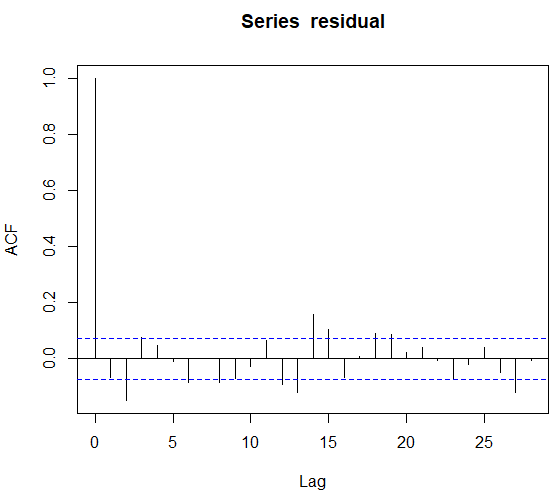
\includegraphics[height=2in]{btcbefno.PNG}
  \caption{ Residual ACF plot for Bitcoin during before period with no penalty}
  \end{subfigure}
% \begin{figure}[h]
  \begin{subfigure}{.49\textwidth}
    \centering
  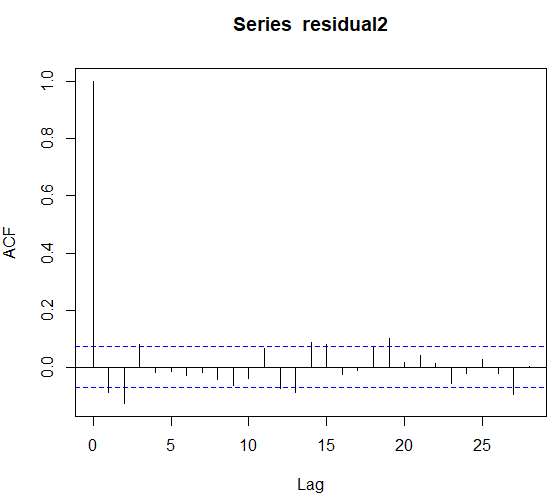
\includegraphics[height=2in]{btcbefstrong.PNG}
  \caption{ Residual ACF plot for Bitcoin during before period with strong penalty}
  \end{subfigure}
  \caption{Residual ACF plot for Bitcoin}
\end{figure}

\begin{figure}[h]
  \begin{subfigure}{.49\textwidth}
    \centering

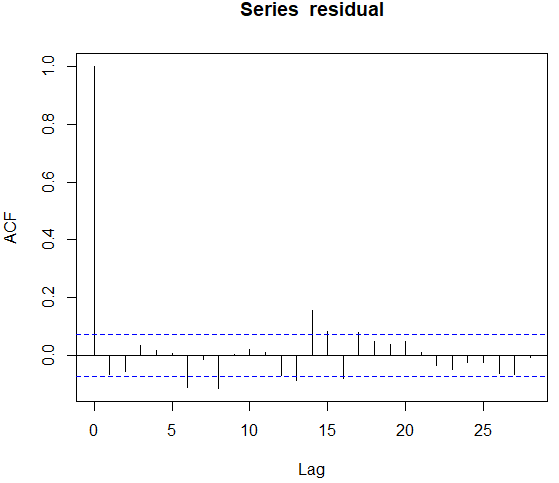
\includegraphics[height=2in]{ethbefno.PNG}
\caption{ Residual ACF plot for Ethereum during before period with no penalty}
  \end{subfigure}
% \begin{figure}[h]
  \begin{subfigure}{.49\textwidth}
  \centering

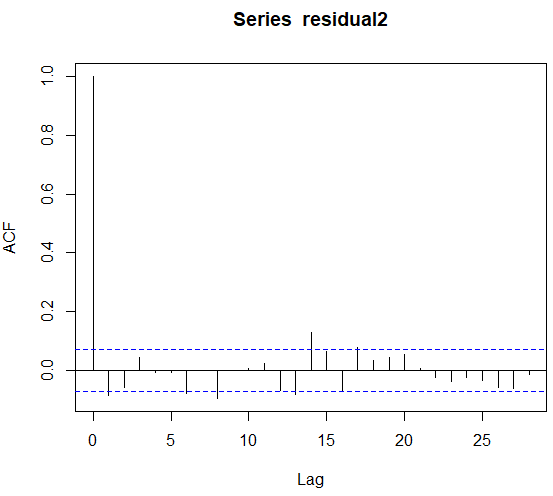
\includegraphics[height=2in]{ethbefstrong.PNG}
\caption{ Residual ACF plot for Ethereum during before period with strong penalty
}
\end{subfigure}
\caption{Residual ACF plot for Ethereum}
\end{figure}




\begin{figure}[h]
  \begin{subfigure}{.49\textwidth}
    \centering
  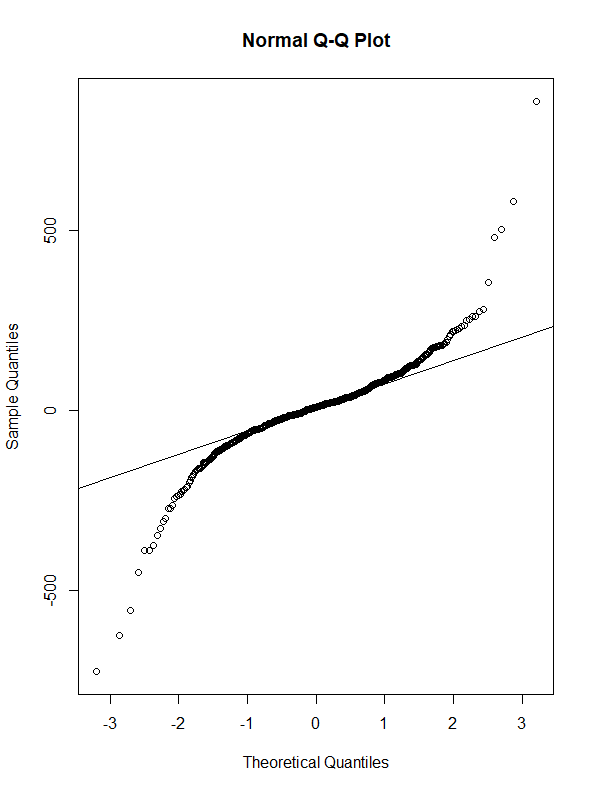
\includegraphics[height=2in]{btcqqbefno.png}
  \caption{ Residual QQ plot for Bitcoin during before period with no penalty}
  \end{subfigure}
% \begin{figure}[h]
  \begin{subfigure}{.49\textwidth}
    \centering
  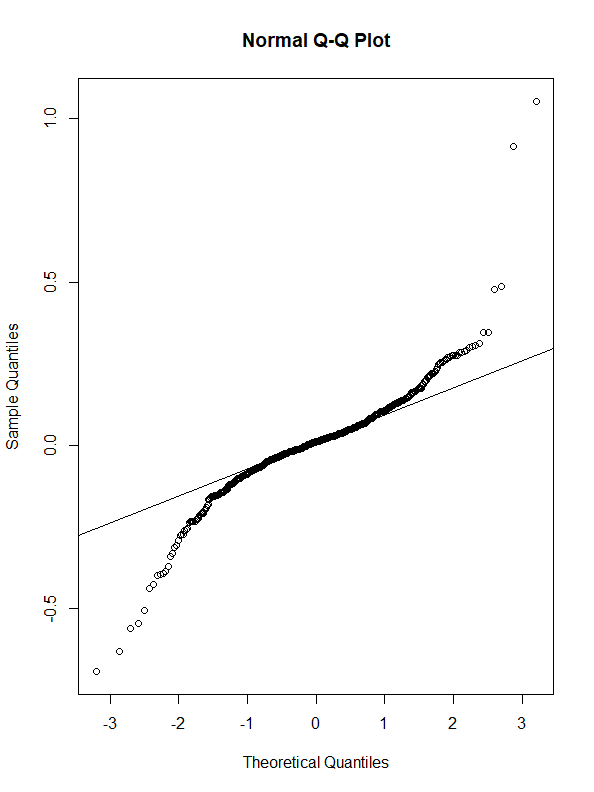
\includegraphics[height=2in]{btcqqbefstrong.png}
  \caption{ Residual QQ plot for Bitcoin during before period with strong penalty}
  \end{subfigure}
  \caption{Residual QQ plot for Bitcoin}
\end{figure}

\begin{figure}[h]
  \begin{subfigure}{.49\textwidth}
    \centering

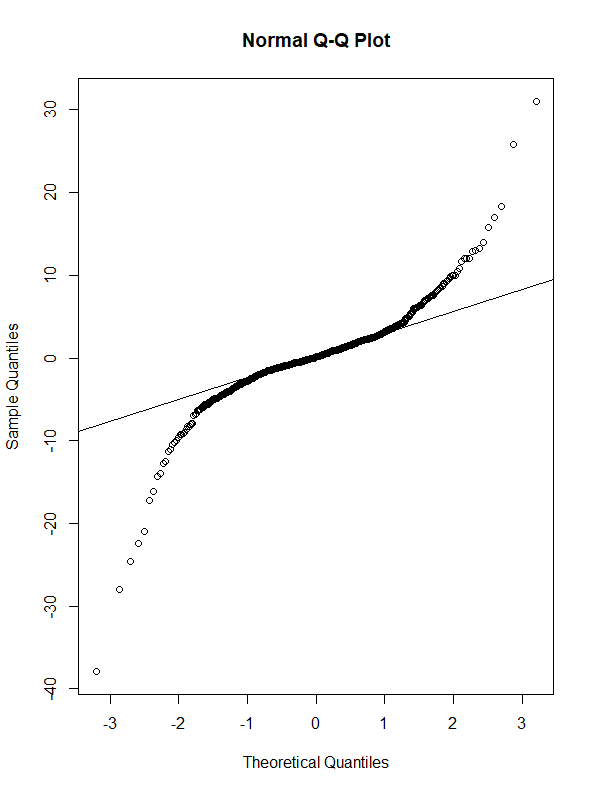
\includegraphics[height=2in]{ethqqbefno.png}
\caption{ Residual QQ plot for Ethereum during before period with no penalty}
  \end{subfigure}
% \begin{figure}[h]
  \begin{subfigure}{.49\textwidth}
  \centering

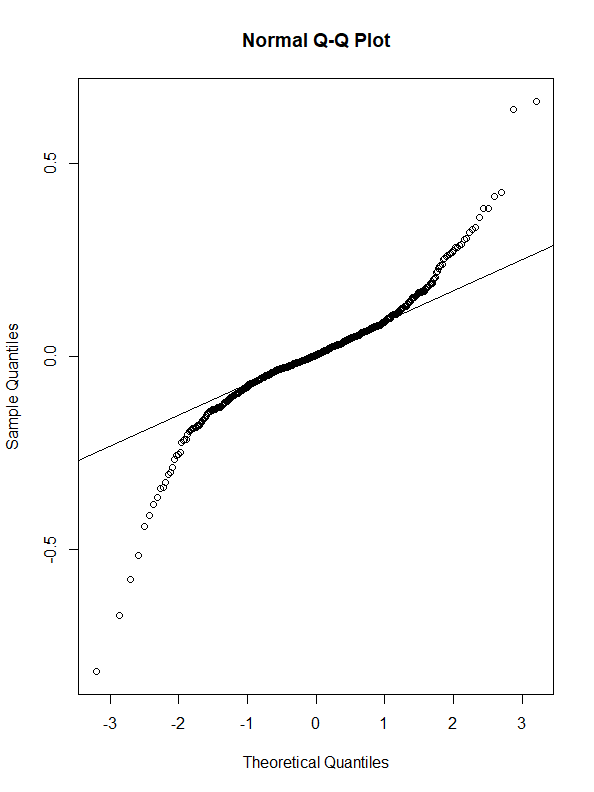
\includegraphics[height=2in]{ethqqbefstrong.png}
\caption{ Residual QQ plot for Ethereum during before period with strong penalty
}
\end{subfigure}
\caption{Residual QQ plot for Ethereum}
\end{figure}

\begin{landscape}
\begin{figure}[h!]
  \caption{Other Parameters}
  \centering
  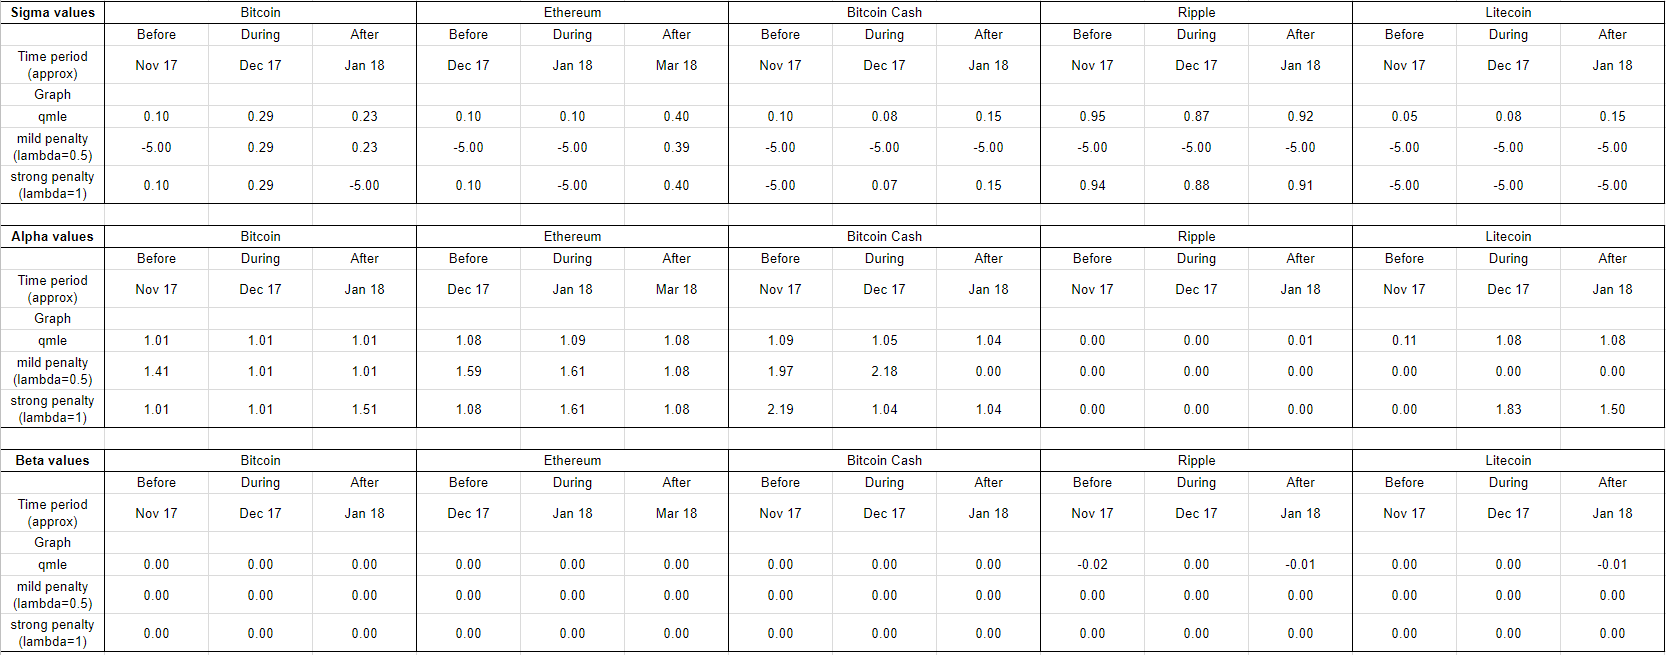
\includegraphics[width=1.4\textwidth]{greeks.PNG}
\end{figure}

\end{landscape}

\end{spacing}
\end{document} to your LaTeX file where you want your
% title page.
%
%%%%%%%%%%%%%%%%%%%%%%%%%%%%%%%%%%%%%%%%%
%\title{Title page with logo}
%----------------------------------------------------------------------------------------
%	PACKAGES AND OTHER DOCUMENT CONFIGURATIONS
%----------------------------------------------------------------------------------------

\documentclass[twocolumns]{IEEEtran} %[xcolor=table]{beamer}%
\usepackage[table]{xcolor}
\usepackage[english]{babel}
\usepackage[utf8x]{inputenc}
\usepackage{amsmath}
\usepackage{graphicx}
\usepackage{setspace}  
\usepackage{lscape}
\usepackage[english]{babel}
\usepackage{subcaption}
% \usepackage{compactenum}
\usepackage[colorinlistoftodos]{todonotes}
% Please add the following required packages to your document preamble:

% If you use beamer only pass "xcolor=table" option, i.e. \documentclass[xcolor=table]{beamer}

\begin{document}

\begin{titlepage}

\newcommand{\HRule}{\rule{\linewidth}{0.5mm}} % Defines a new command for the horizontal lines, change thickness here

\center % Center everything on the page
 
%----------------------------------------------------------------------------------------
%	HEADING SECTIONS
%----------------------------------------------------------------------------------------

\textsc{\LARGE Cornell University}\\[1.5cm] % Name of your university/college
\begin{figure}
  \centering
  
\includegraphics[width=0.25\textwidth]{cornell.png}
\end{figure}

\textsc{\Large ORIE 5640}\\[0.5cm] % Major heading such as course name
\textsc{\large Statistics for Financial Engineering}\\[0.5cm] % Minor heading such as course title

%----------------------------------------------------------------------------------------
%	TITLE SECTION
%----------------------------------------------------------------------------------------

\HRule \\[0.4cm]
{ \huge \bfseries Bubble Detection for Cryptocurrency }\\[0.4cm] % Title of your document
\HRule \\[1.5cm]
 
%----------------------------------------------------------------------------------------
%	AUTHOR SECTION
%----------------------------------------------------------------------------------------

\begin{minipage}{0.4\textwidth}
\begin{flushleft} \large
\emph{Author:}\\
Chen \textsc{Zhong} \\
Chen \textsc{Weijia} \\
Yi \textsc{Shen} \\
Chen \textsc{Peng Yuan} \\

% Your name
\end{flushleft}
\end{minipage}
~
\begin{minipage}{0.4\textwidth}
\begin{flushright} \large
\emph{Professor:} \\
Prof. Edward \textsc{Mehrez} % Supervisor's Name
\end{flushright}
\end{minipage}\\[2cm]

% If you don't want a supervisor, uncomment the two lines below and remove the section above
%\Large \emph{Author:}\\
%John \textsc{Smith}\\[3cm] % Your name

%----------------------------------------------------------------------------------------
%	DATE SECTION
%----------------------------------------------------------------------------------------

{\large May 21, 2018}\\[2cm] % Date, change the \today to a set date if you want to be precise
 
%----------------------------------------------------------------------------------------

\vfill % Fill the rest of the page with whitespace

\end{titlepage}
\onecolumn
\setcounter{tocdepth}{2}
\tableofcontents
\clearpage


\begin{spacing}{1.5}
\begin{abstract}
Since the 2000 dot-com bubble and the 2008-2009 financial crisis, bubbles became an essential issue among the financial industry. Within the past few years, cryptocurrency emerged as a popular asset not only among institutional investors, but also among the retail investors. The problem that we are going to address is to determine in real time whether different cryptocurrencies exhibit a bubble, which has the characteristic of reaching unrealistic price level and then crashes. Our procedure involves Lasso estimation and using the standard stochastic differential equation driven by a Brownian motion to determine whether the process is a strict local martingale. We will illustrate this bubble detection procedure by applying on the cryptocurrency asset class, where we believe price bubbles were widely thought to have existed.
\end{abstract}

\section{Introduction}
Crypotocurrencies became a heated topic recently. Cryptocurrencies had become all over the financial news. In 2008, pseudonymous Satoshi Nakamoto introduced the digital decentralized cryptocurrency, bitcoin. Since then, people have envisioned cryptocurrency as the next generation of currency. Bitcoin has experienced the super-exponential growth. Due to the rise of the popularity of bitcoin, other cryptocurrencies also erupted into the mainstream. This creates a popular demand among all the investors, from institutional investors to retail investors. Cryptocurrencies have become an emerging asset class. At the end of 2017, the price of bitcoin peaked at almost 20,000 USD, and the combined market capitalization of cryptocurrencies reached around 800 billion USD.

Conventional view is that asset bubbles are rare. However, we believe that there are bubbles among the cryptocurrencies. For a bubble to develop among an asset class, first the asset class will start to be in an overheated market in which there are too many buyers who are too keen to buy. As a result, prices rise way too fast, and this situation becomes unsustainable. Eventually, some people realize this and start to sell out of the asset. The whole process goes into reverse equally rapidly, and the bubble bursts. This caused all the people to sell in panic so that prices plunge rapidly. Some of the intuitions behind the finance bubble are when retail investors start to talk about it, the media and news start to cover about the asset class all over the place. However, these are fundamental views without mathematical theory proofs. 

In this paper, we are concentrating on detecting bubbles in cryptocurrencies, including Bitcoin, Bitcoin Cash, Ripples, Litecoin and Ethereum. Our procedure involved using the standard stochastic differential equation driven by a Brownian Motion to determine whether the process is a strict local martingale using QMLE and Lasso estimation.

\section{Bubble Theory}
As shown by Jarrow, Protter and Shimbo\cite{jarrow2011detect}, there are mainly three types of asset price bubbles. Among them, two exist in infinite horizon economies under the weakly complete market which is frictionless, competitive and continuous trading. Hence, we consider the Type Three Bubbles, which exist in finite horizons. According to their theory, a model for asset price process using a  standard stochastic differential equation driven by a Brownian Motion is given as below:
$$dS_t=\sigma(S_t)dW_t+\mu(S_t)dt$$
Under No-arbitrage setting, there exists risk neutral measure under which the SDE satisfies this:
$$S_t=S_0+\int_0^t\sigma(S_s)dW_s$$
whether this type of bubbles exists or not is determined by whether the price process under risk-neutral measure is a strict local martingale. 

\subsection{Theory}
A stochastic process $M = (M_n)_{n\ge n}$ with the relation that $E(M_m|F_n)=M_n$ for any $m\ge n$ is called a martingale.

Here, martingale means a process whose expected future values equals its present value, conditioned on history. The intuition behind the distinction between a martingale and a strict local martingale (in the case where the local martingale $S > 0$) derived from the fact that local martingale is always a supermartingale, which has a decreasing trend in the future expected value. The local martingale is a martingale if and only if it has constant expectation. 

Whether this type of bubbles exists or not is determined by whether the price process under risk-neutral measure is a strict local martingale. More formally, through Comparison Theorem*, we have Type Three Bubbles exist if and only if,
$$\int_{\alpha}^{\infty}\frac{x}{\sigma^2(x)}dx<\infty$$
for all $\alpha>0.$  
\subsection{Intuition}
$$
P_t > E^{Q}  [e^{-r (\tau - t)} P_{\tau} ]
$$
where $P_{\tau}$ is the liquidation value at time $\tau$.

The economic intuition behind this is that the present price is greater than expected future cash flows under the risk neutral measure. According to the fundamental theorem of asset pricing, current price of an asset should be equal to the discounted future cash flow under the risk neutral measure. When price at time t is greater than that value we call it a super martingale. This indicates that the current price of the asset is greater than what the fundamentals of the asset suggests, and that people are not trading on the intrinsic value but on the certain unrealistic expectation, hence the bubble.



\section{Model Selection}
We now consider a proper way to apply the bubble theory to our cryptocurrency data. As implied above in the bubble theory, according to the comparison theorem we need a parametric model for the diffusion term in order to calculate the integral. Hence our objective here is to fit our data to an appropriate parametric model so we can use the parameters derived to perform the bubble test.\\
For the specific methods to fit our data with, we will be considering the following parametric model fitting processes:
\begin{itemize}
\item QMLE (Quasi-Maximum Likelihood Estimator)
\item LASSO (Least Absolute Shrinkage and Selection Operator)
\end{itemize}
\subsection{Base Model}
Consider the following stochastic differential equation;
$$
dX_t = b(\theta_2,X_t)dt+\sigma(\theta_1,X_t)dW_t
$$

This is the most general form of stochastic process to model any kind of price process. Function $b$ is a deterministic function with parameters $\theta_2$ and the  asset price at time $t$, function $\sigma$ is also a deterministic function with parameters $\theta_1$ and asset price. This structure has the flexibility to capture most potential behaviors of cryptocurrencies.

We will determine the precise model to fit our data with later.

\subsection{QMLE}
QMLE stands for Quasi-Maximum Likelihood Estimator, it is a method to estimate parameters of a statistical model very similar to MLE
(Maximum Likelihood Estimator). Both methods choose the parameters that maximize the likelihood function. MLE maximizes the log likelihood function while QMLE maximizes a function that is similar to the log likelihood function but has a simpler version in structure.

The pro of using QMLE is that it specifies a density function that admits specifications of different conditional moments and other distribution characteristics. The con is that it introduces misspecification errors. Hence QMLE requires careful construction of the likelihood function to avoid these errors.

In order to implement QMLE, we need to compare the difference in information presented by the original MLE likelihood and the QMLE approximated likelihood. Here we consider the Kullback-Leibler Information Criterion(KLIC) of $g$ relative to $f$ as: 
$$
 \mathbf{I} (g:f) = \int_{\mathbf{R}} log(\frac{g(\xi)}{f(\xi)})g(\xi)d\xi
$$

KLIC is the rough measure of the closeness between f and g. To approximate $g_t(y_t|x_t)$, we specify a quasi-likelihood function $f_t(y_t|x_t;\theta)$. KLIC of $g_t$ relative to $f_t$ is:
$$
 \mathbf{I} (g_t:f_t;\theta) = \int_{\mathbf{R}} log(\frac{g_t(y_t|x_t)}{f_t(y_t|x_t;\theta)})g_t(y_t|x_t)dy_t
$$

For a sample of T observations we consider the average of T individual KLICs:

$$
 \bar{\mathbf{I}}_T (g_t:f_t;\theta) = \frac{1}{T} \sum_{t=1}^{T}\mathbf{I}(g_t:f_t;\theta)=\frac{1}{T} \sum_{t=1}^{T}(\mathbf{E}[log\,g_t(y_t|x_t)]-\mathbf{E}[log\, f_t(y_t|x_t;\theta)])
$$

We wish to minimize the total KLIC to get a close estimate, hence we need to maximize:

$$
\bar{L}_T(\theta)=\frac{1}{T}\sum_{t = 1}^{T}\mathbf{E}[log\, f_t(y_t|x_t;\theta)]
$$

Since it is not directly observable due to the expectation, in practice, we will try to maximize its sample counterpart:

$$
L_T(y^T,x^T;\theta)=\frac{1}{T}\sum_{t = 1}^{T}log\, f_t(y_t|x_t;\theta)
$$

The resulting $\theta$ will be our quasi-maximum likelihood estimator.

For diffusion process solutions of SDE and observed at discrete times such as our model, we can define the likelihood function using the Markov property. First we can construct the likelihood function $L_n(\theta)$ of the Markovian process X using the conditional distributions:

$$
L_n(\theta) = \prod_{i=1}^{n}p_{\theta}(\Delta_i,X_i|X_{i-1})p_{\theta}(X_0)
$$

Assuming $p_{\theta}(X_0)=1$ and take log to the likelihood function we get a log-likelihood function:

$$
l_n(\theta)=log\,L_n(\theta)=\sum_{i=1}^n l_i(\theta)+log(p_{\theta}(X_0))=\sum_{i=1}^n log\,p_{\theta}(\Delta_i,X_i |X_{i-1})
$$

Since exact likelihood inference is not always possible, explicit form of the function is rarely known. For parameters in the diffusion coefficient, MLE rate of convergence if order $\sqrt{n}$ while the estimators for the drift convergence is of order $\sqrt{T}$. Hence we require $n\Delta=T \to \infty$. Using the Euler-Maruyama discretization scheme as introduced by the work of Genon-Catalot and Jacod(1993) we get our approximated negative log likelihood function:

$$
l_n(X_n,\theta) = -\frac{1}{2}\sum_{i=1}^{n}\{ log \,\textbf{det}(\sigma_{i-1}(\theta_1)) + \frac{1}{\Delta_n}\Sigma_{i-1}^{-1}(\theta_1)[\Delta X_i-\Delta_n b_{i-1}(\theta_2)]^{\otimes 2} \}
$$

Where $\theta=(\theta_1,\theta_2),\, \Delta X_i = X_{t_i}-X_{t_{i-1}},\, \Sigma_i(\theta_1) = \Sigma(\theta_1,X_t),\, b_i(\theta_2)=b(\theta_2,X_{t_i}),\, \Sigma=\sigma^{\otimes 2},\, A^{\otimes 2}=A^TA$, and $A^{-1}$ the inverse of A, then the QML estimator of $\theta$ is:

$$
\tilde{\theta}_n = arg\min_{\theta}\, l_n(X_n,\theta)
$$

Notice here that the sign for the likelihood function is negative, which turns the argmin function to maximization. The approximate log-likelihood function consists of 2 parts: stochastic volatility term, and the standardized price change term. This approximate function has the characteristics of log likelihood and certainly components of other model specifications as well.

In our case, we will be using the built-in solver from the Yuima package which uses the contrast function from the work of Genon-Catalot and Jacod \cite{genon1993estimation}.

\subsection{LASSO}
On top of QMLE, we will also be applying LASSO (least absolute shrinkage and selection operator) as an improvement to the parameter selection process. It is a regression analysis method that performs both variable selection and regularization. LASSO can enhance prediction accuracy and interpretability by streamlining the selection of variables and highlight the more significant ones. It does so by putting constraints on parameters, and introduces regularizers, the argmin function will try to minimize the number and size of coefficients while maintaining the efficiency of the results.

Using LASSO is very useful for models with many parameters since it can eliminate unnecessary coefficients. It is also useful in our implementation since we aim at modeling with a general model, with too many parameters, we might risk over fitting our data. Hence LASSO is very useful for modeling in our case to eliminate unnecessary parameters, even when there are only a few we still want to choose the most significant ones.

QMLE + LASSO parameter selection function:

$$
\min l_n(X_n,\theta)+ \sum^p_{j=1}\lambda_{n,j} |\theta_{2j}| + \sum^q_{k = 1}\gamma_{n,k} |\theta_{1k}|
$$

The minimization problem (maximization for the log likelihood) here aims at finding the parameters that maximizes the QMLE function while keeping the LASSO terms minimum. 

Depending on the sensitivity towards the size of parameter, we will have 3 different degrees of penalty settings as a parameter on LASSO:
\begin{itemize}
\item No penalty: no LASSO term in the function, only the QMLE term
\item Mild penalty: small penalty on magnitude of parameters, decrease the occurrence of large parameters, prevents collinearity of variables
\item Strong penalty: big penalty on magnitude of parameters, eliminate the occurrence of large parameters
\end{itemize}

\subsection{CKLS Model}
Since we don't know the exact property of cryptocurrency price changes, the best approximation is to treat them like asset price. Our simplest model for stock price is geometric brownian motion (GBM), and a good model for short term interest rate is the Vasicek short rate model, and there are a lot more to choose from. We want something that has enough flexibility to describe a variety of characteristic to allow for generality.

Chan, Karolyi, Longstaff and Sanders (CKLS) achieves just that:
$$
dX_t = (\alpha + \beta X_t)dt + \sigma X_t^{\gamma}dW_t
$$

By modifying the parameters, it can become Merton model, Vasicek model, Cox model, GBM model and many more. It has the flexibility to describe the behavior of cryptocurrency.

More importantly, the diffusion term is a power function: $\sigma X_t^{\gamma}$, whose $\gamma$ parameter is the indicator for the bubble test
\subsection{Bubble Test}
As mentioned in the bubble theory, we want to test whether $\int^{\infty}_{\alpha}\frac{x}{\sigma^2(x)}dx < \infty$.

Substitute $\sigma (x)$ with $\sigma x^{\gamma}$:

\begin{equation}
\begin{aligned}
\int^{\infty}_{\alpha}\frac{x}{\sigma^2(x)}dx &= \int^{\infty}_{\alpha}\frac{x}{(\sigma x^{\gamma})^2}dx \\
&= \frac{1}{\sigma^2}\int^{\infty}_{\alpha}\frac{x}{x^{2\gamma}}dx \\
&= \frac{1}{\sigma^2}\int^{\infty}_{\alpha}x^{1-2\gamma}dx \\
&= \frac{1}{\sigma^2}\frac{1}{2-2\gamma}x^{2-2\gamma} |_{\alpha}^{\infty}
\end{aligned}
\end{equation}

Integral goes to infinity if and only if $\gamma > 1$, hence according to comparison theorem, the process X is:
\begin{itemize}
\item a strict local martingale if $\gamma > 1$ (bubble)
\item a martingale if $\gamma \le 1$ (not bubble)
\end{itemize}

\section{Evaluation}

We evaluated the model based on five major cryptocurrencies during three manually selected periods: before the bubble appears (when the price soars), during the bubble happens (when the price remain high), and after the bubble bursts (when the price plummets). We expect to see that our model output that there is a bubble during the first period, and not a bubble after the second period. 

For each period, we used plain QMLE method, QMLE with mild LASSO regularization and QMLE with strong LASSO regularization to evaluate the $\gamma$ parameters. 

At the end of this paper is a table of results we generated using the YUIMA package \cite{brouste2013parameter}. 

From the result (as shown in table I) along with our other observations, we come up with the following findings:

\subsection{Effect of model}
\begin{enumerate}
\item All the estimation methods generate expected results ($\gamma>1$) for ``before the bubble'' period for all the cryptocurrencies. 
\item For estimations of ``during the bubble'' periods, we are more likely to have $\gamma>1$ when a sudden spike of price is included in that period.
\item Our estimation for gamma in ``during the bubble'' and ``after the bubble'' periods vary, while the plain QMLE methods generates desirable results.  
\end{enumerate}

\subsection{Robustness of estimator}
Significant ourliers in the table can be observed in the evaluation for Ripple, where the estimated $\gamma$ are around zero for before and after the bubble periods. A significant difference between ripple and other cryptocurrencies is that its price is considerably low ($<$\$5) throughout the whole period, compared with some thousand dollars of value for cryptos like bitcoin and bitcoin cash. Therefore, we suspect that the value of the price could influence the performance of our model. We therefore added a big constant (1000) to the Ripple prices and evaluated it using the model and the $\gamma$ we got then all exceed 1. Though a rough method, it somehow indicates that the stability of such a model might be a concern and preprocessing the data using some normalization technique might be helpful.

\subsection{Effect of LASSO regularizer}

It is quite surprise to the author that the estimated values generated by adding the LASSO regularizer to the plain QMLE method is quite large. This not only true for the $\gamma$ value, but also for total sum of absolute value of $\alpha, \beta, \gamma$ and $\sigma$ in the model, which goes against our motive for adding such a regularizer. Intuitively, LASSO regularizer applies to a model with many (perhaps hundreds or thousands of) parameters where we wish to have most of the parameters close to zero and a few comparatively large values. The CKLS model only have 4 parameters --- $\alpha, \beta, \gamma$ and $\sigma$, all of which contain significant information of the model. The author thus doubts the effect of applying the LASSO regularizer to such a model, given the unexpected results.

\subsection{Higher frequency data}

We also implemented the evaluation for higher frequency data (minute data for 1-2 weeks) but got some quite disappointing results. All the estimators render $\gamma\geq1$ for all periods and all cryptocurrencies. We doubt that such a model might be prone to noises in high frequency data and thus decide not to reveal the results.  

\subsection{Robustness: Window Extension}
In previous results, we set our time window separately for the before, during and after periods. We wonder if our test will yield more interesting result if we run our test with cumulative data. As shown in table II, we ran our test using cumulative data in the before period and the before and during period.

We are most interested in the before and during period. When we run our test with cumulative data, all parameters except for that of Ripple's are greater than 1, meaning all asset show sign of bubble when we run the cumulative data up to when the suspected bubble burst.

\subsection{Specification Test}
In order to test whether CKLS model is indeed a good fit for the cryptocurrency market, we need to check the standardized residual:
$$
\epsilon_t = \frac{\Delta S_t-\hat{b}(\alpha,\beta,S_{t-1})\Delta_t}{\hat{\sigma}(\sigma,S_{t-1})}
$$

If our model is a good fit then: $\epsilon_t \approx \Delta W_t \sim N(0,\Delta_t)$.
\subsubsection{ACF-plot}
The residuals from our model should be stationary series. From ACF plots of residuals (Fig.1-2) we can see that there are no significant spikes, meaning the residuals are stationary and that the resulting model is a decent fit for our data, and any potential issue of the model might stem from the implementation procedure.
\subsubsection{QQ-plot}
As shown in the QQ-plot (Fig.3-4), the standardized residuals are not exactly normally distributed, but all of them have heavier tails than the normal distribution. The deviation from the normal are very much even on both ends, meaning the distribution is not skewed to one side. This is an evidence that standard Brownian Motion may not be the fundamental drive of the bubble price process. As an indication for future work, this means that instead of modeling using normal distribution, we can assume that the distribution is t-distribution and base our model on t-distribution, which can adjust for the heavier tail. 
\section{Conclusion}
In this project, we studied the bubble theory \cite{jarrow2011detect} proposed by Jarrow, Kchia, and Protter and analyzed the mathematics behind such theory, We selected CKLS stochastic model for evaluation and implemented it on 5 major cryptocurrencies prices at the end of 2017 when we witness significantly soaring prices. The quasi-maximum likelihood estimator generates remarkable results for bubble detection while the effect of LASSO regularizer is less desirable.

\bibliographystyle{unsrt}
\bibliography{ref}

\begin{landscape}
\begin{table}[]
\centering
\resizebox{\textwidth}{!}{%
\begin{tabular}{|c|ccc|ccc|ccc|ccc|ccc|}
\hline
Gamma values & \multicolumn{3}{c|}{Bitcoin} & \multicolumn{3}{c|}{Ethereum} & \multicolumn{3}{c|}{Bitcoin Cash} & \multicolumn{3}{c|}{Ripple} & \multicolumn{3}{c|}{Litecoin} \\ \hline
 & \multicolumn{1}{c|}{Before} & \multicolumn{1}{c|}{During} & After & \multicolumn{1}{c|}{Before} & \multicolumn{1}{c|}{During} & After & \multicolumn{1}{c|}{Before} & \multicolumn{1}{c|}{During} & After & \multicolumn{1}{c|}{Before} & \multicolumn{1}{c|}{During} & After & \multicolumn{1}{c|}{Before} & \multicolumn{1}{c|}{During} & After \\ \hline
Time period (approx) & \multicolumn{1}{c|}{Nov 17} & \multicolumn{1}{c|}{Dec 17} & Jan 18 & \multicolumn{1}{c|}{Dec 17} & \multicolumn{1}{c|}{Jan 18} & Mar 18 & \multicolumn{1}{c|}{Nov 17} & \multicolumn{1}{c|}{Dec 17} & Jan 18 & \multicolumn{1}{c|}{Nov 17} & \multicolumn{1}{c|}{Dec 17} & Jan 18 & \multicolumn{1}{c|}{Nov 17} & \multicolumn{1}{c|}{Dec 17} & Jan 18 \\ \hline
qmle & 1.000 & 0.890 & 0.910 & 1.000 & 0.806 & 0.797 & 1.010 & 1.040 & 0.950 & -0.010 & -0.135 & -0.087 & 1.120 & 1.030 & 0.920 \\ \cline{1-1}
\rowcolor[HTML]{C0C0C0} 
std.qmle & 0.021 & 0.013 & 0.016 & 0.021 & 0.017 & 0.008 & 0.011 & 0.011 & 0.016 & 9.211 & 0.420 & 6.490 & 0.035 & 0.017 & 0.023 \\ \cline{1-1}
mild penalty ($\lambda$=0.5) & 6.655 & 0.890 & 0.910 & 8.000 & 0.806 & 2.937 & 8.000 & 8.000 & 5.526 & 0.000 & 4.677 & 0.000 & 8.000 & 8.000 & 7.630 \\ \cline{1-1}
\rowcolor[HTML]{C0C0C0} 
std.qmle & 0.015 & 0.009 & 0.011 & 0.015 & 0.012 & 0.006 & 0.008 & 0.008 & 0.011 & 0.003 & 0.297 & 0.005 & 0.025 & 0.012 & 0.016 \\ \cline{1-1}
strong penalty ($\lambda$=1) & 1.000 & 0.890 & 3.300 & 8.000 & 0.806 & 0.795 & 8.000 & 1.040 & 0.949 & 0.000 & 0.476 & 0.000 & 8.000 & 8.000 & 7.630 \\ \cline{1-1}
\rowcolor[HTML]{C0C0C0} 
std.qmle & 0.015 & 0.009 & 0.011 & 0.015 & 0.012 & 0.006 & 0.008 & 0.008 & 0.011 & 0.001 & 0.297 & 0.003 & 0.025 & 0.012 & 0.016 \\ \hline
\end{tabular}
}
\caption{Estimated $\gamma$ and its standard deviation for different cryptocurrencies in different periods. ($\lambda$ $\text{ indicates the shrinkage level.}$)}

\label{result}
\end{table}

\begin{table}[]
\centering

\resizebox{\textwidth}{!}{%
\begin{tabular}{|c|cc|cc|cc|cc|cc|}
\hline
Gamma values              & \multicolumn{2}{c|}{Bitcoin}         & \multicolumn{2}{c|}{Ethereum}        & \multicolumn{2}{c|}{Bitcoin Cash}    & \multicolumn{2}{c|}{Ripple}          & \multicolumn{2}{c|}{Litecoin}        \\ \hline
& \multicolumn{1}{c|}{Before} & Before \& During & \multicolumn{1}{c|}{Before} & Before \& During & \multicolumn{1}{c|}{Before} & Before \& During
& \multicolumn{1}{c|}{Before} & Before \& During & \multicolumn{1}{c|}{Before} & Before \& During\\ \hline
Time period (approx)      
& \multicolumn{1}{c|}{Nov 17} & Nov-Dec 17 & \multicolumn{1}{c|}{Dec 17} & Dec 17-Jan 18 & \multicolumn{1}{c|}{Nov 17} & Nov-Dec 17& \multicolumn{1}{c|}{Nov 17} & Nov-Dec 17 & \multicolumn{1}{c|}{Nov 17} & Nov-Dec 17 \\ \hline
qmle   & 1.000    & 1.001  & 1.000    & 1.028& 1.011    & 1.009  & -0.010   & -0.067 & 1.130    & 1.103  \\ \cline{1-1}
\rowcolor[HTML]{C0C0C0} 
std.qmle   & 0.021    & 0.021  & 0.035    & 0.018  & 0.011    & 0.008  & 9.211    & 1.045  & 0.035    & 0.015  \\ \cline{1-1}
mild penalty ($\lambda$=0.5) & 6.655    & 8.000  & 8.000    & 8.000  & 8.000    & 7.922  & 0.000   & 0.000  & 8.000    & 8.000  \\ \cline{1-1}
\rowcolor[HTML]{C0C0C0} 
std.qmle  & 0.015    & 0.015  & 0.025    & 0.013  & 0.008    & 0.005  & 0.003    & 0.005  & 0.025    & 0.011  \\ \cline{1-1}
strong penalty ($\lambda$=1) & 1.000    & 8.000  & 0.997    & 8.000  & 8.000    & 1.008  & 0.000    & -0.065  & 8.000    & 8.000  \\ \cline{1-1}
\rowcolor[HTML]{C0C0C0} 
std.qmle  & 0.015    & 0.015  & 0.025    & 0.013  & 0.008    & 0.005  & 0.001    & 0.739  & 0.025    & 0.011  \\ \hline
\end{tabular}%
}
\label{my-label}
\caption{Estimated $\gamma$ and its standard deviation for different cryptocurrencies in before and before/during periods. ($\lambda$ $\text{ indicates the shrinkage level.}$)}
\end{table}
% \begin{table}[]
% \centering
% \begin{tabular}{|c|ccc|ccc|ccc|ccc|ccc|}
% \hline
% Gamma values & \multicolumn{3}{c|}{Bitcoin} & \multicolumn{3}{c|}{Ethereum} & \multicolumn{3}{c|}{Bitcoin Cash} & \multicolumn{3}{c|}{Ripple} & \multicolumn{3}{c|}{Litecoin} \\ \hline
%  & \multicolumn{1}{c|}{Before} & \multicolumn{1}{c|}{During} & After & \multicolumn{1}{c|}{Before} & \multicolumn{1}{c|}{During} & After & \multicolumn{1}{c|}{Before} & \multicolumn{1}{c|}{During} & After & \multicolumn{1}{c|}{Before} & \multicolumn{1}{c|}{During} & After & \multicolumn{1}{c|}{Before} & \multicolumn{1}{c|}{During} & After \\ \hline
% Time period (approx) & \multicolumn{1}{c|}{Nov} & \multicolumn{1}{c|}{Nov-Dec} & Nov-Jan & \multicolumn{1}{c|}{Nov} & \multicolumn{1}{c|}{Nov-Dec} & Nov-Jan & \multicolumn{1}{c|}{Nov} & \multicolumn{1}{c|}{Nov-Dec} & Nov-Jan & \multicolumn{1}{c|}{Nov} & \multicolumn{1}{c|}{Nov-Dec} & Nov-Jan & \multicolumn{1}{c|}{Nov} & \multicolumn{1}{c|}{Nov-Dec} & Nov-Jan \\ \hline
% qmle 
% & 1.000 & 1.001 & 1.001 & 0.999 & 1.028 & 1.022 & 1.011 & 1.009 & 0.987 & -0.019 & -0.067 & -0.084 & 1.130 & 1.103 & 1.090 \\ \cline{1-1}
% \rowcolor[HTML]{C0C0C0} 
% std.qmle 
% & 0.021 & 0.011 & 0.009 & 0.035 & 0.018 & 0.013 & 0.011 & 0.008 & 0.007 & 4.835 & 1.045 & 0.429 & 0.035 & 0.015 & 0.013 \\ \cline{1-1}
% mild penalty ($\lambda$=0.5) 
% & 6.655 & 6.385 & 6.391 & 8.000 & 8.000 & 8.000 & 8.000 & 7.922 & 0.986 & -4.944 & 0.000 & 8.000 & 8.000 & 8.000 & 8.000 \\ \cline{1-1}
% \rowcolor[HTML]{C0C0C0} 
% std.qmle 
% & 0.015 & 0.008 & 0.007 & 0.025 & 0.013 & 0.009 & 0.008 & 0.005 & 0.005 & 0.004 & 0.005 & 0.303 & 0.025 & 0.011 & 0.009 \\ \cline{1-1}
% strong penalty ($\lambda$=1)
% & 1.000 & 1.000 & 1.000 & 0.997 & 8.000 & 8.000 & 8.000 & 1.001 & 6.945 & 2.437 & -0.065 & 0.070 & 8.000 & 8.000 & 8.000 \\ \cline{1-1}
% \rowcolor[HTML]{C0C0C0} 
% std.qmle 
% & 0.015 & 0.008 & 0.007 & 0.025 & 0.013 & 0.009 & 0.008 & 0.005 & 0.005 & 0.001 & 0.739 & 0.303 & 0.025 & 0.011 & 0.009 \\ \hline
% \end{tabular}
% \caption{Estimated $\gamma$ and its standard deviation for different cryptocurrencies in different periods.(cumulative) ($\lambda$ $\text{ indicates the shrinkage level.}$)}

% \label{result}
% \end{table}
\end{landscape}

\begin{figure}[h]
  \begin{subfigure}{.49\textwidth}
    \centering
  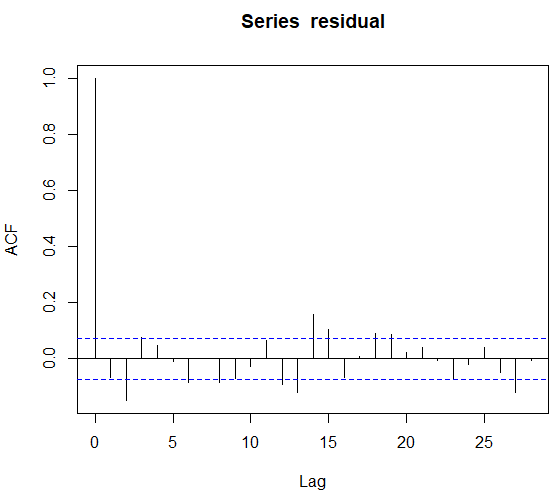
\includegraphics[height=2in]{btcbefno.PNG}
  \caption{ Residual ACF plot for Bitcoin during before period with no penalty}
  \end{subfigure}
% \begin{figure}[h]
  \begin{subfigure}{.49\textwidth}
    \centering
  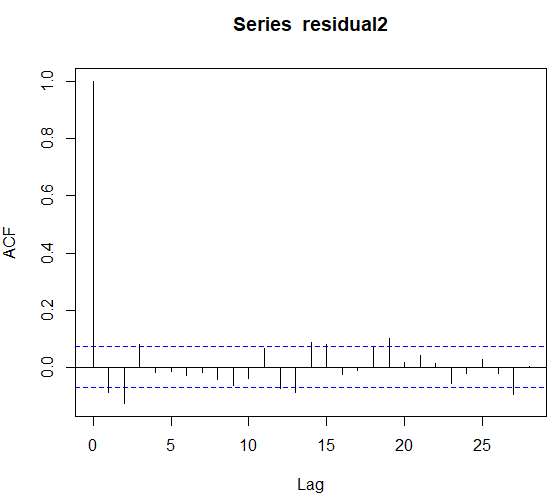
\includegraphics[height=2in]{btcbefstrong.PNG}
  \caption{ Residual ACF plot for Bitcoin during before period with strong penalty}
  \end{subfigure}
  \caption{Residual ACF plot for Bitcoin}
\end{figure}

\begin{figure}[h]
  \begin{subfigure}{.49\textwidth}
    \centering

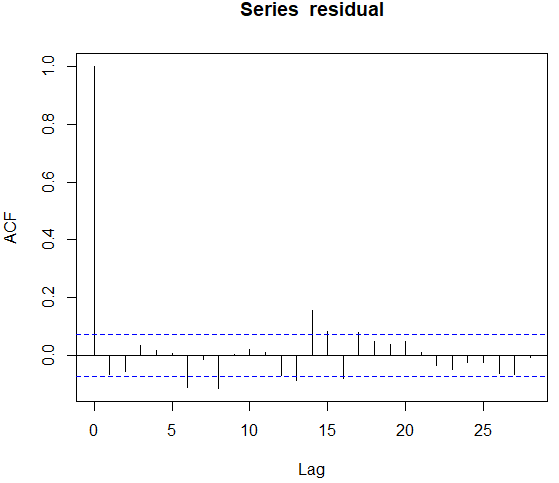
\includegraphics[height=2in]{ethbefno.PNG}
\caption{ Residual ACF plot for Ethereum during before period with no penalty}
  \end{subfigure}
% \begin{figure}[h]
  \begin{subfigure}{.49\textwidth}
  \centering

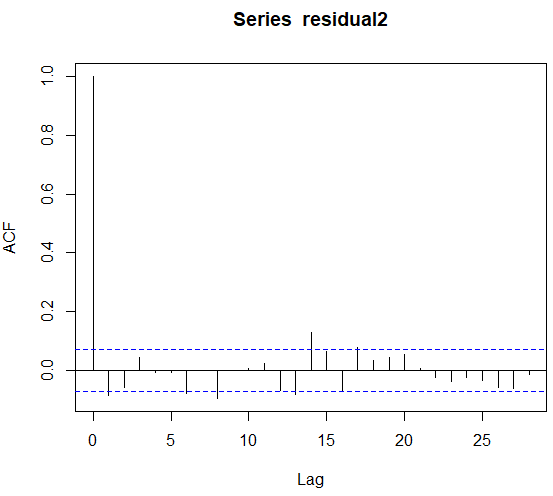
\includegraphics[height=2in]{ethbefstrong.PNG}
\caption{ Residual ACF plot for Ethereum during before period with strong penalty
}
\end{subfigure}
\caption{Residual ACF plot for Ethereum}
\end{figure}




\begin{figure}[h]
  \begin{subfigure}{.49\textwidth}
    \centering
  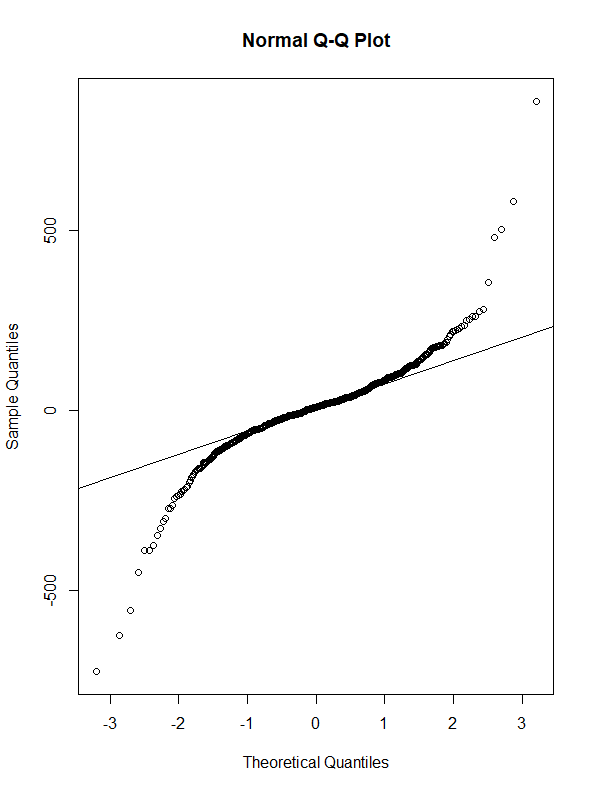
\includegraphics[height=2in]{btcqqbefno.png}
  \caption{ Residual QQ plot for Bitcoin during before period with no penalty}
  \end{subfigure}
% \begin{figure}[h]
  \begin{subfigure}{.49\textwidth}
    \centering
  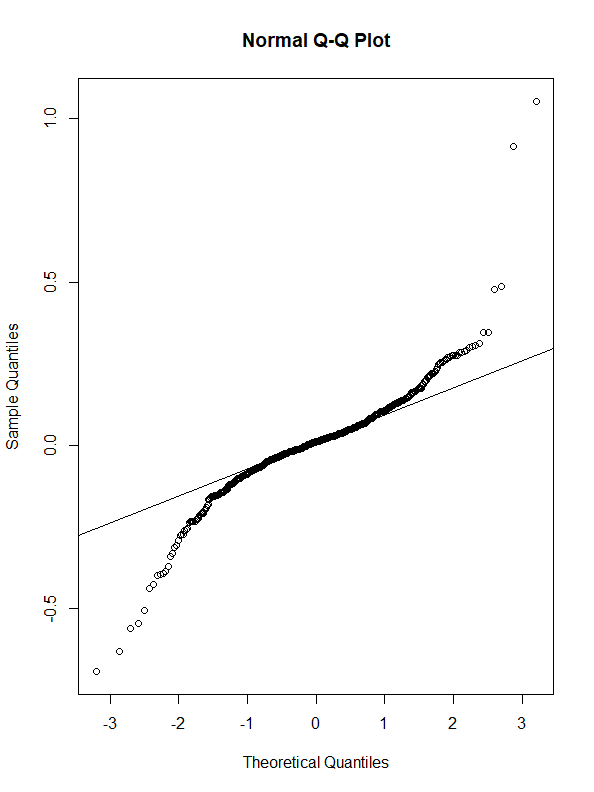
\includegraphics[height=2in]{btcqqbefstrong.png}
  \caption{ Residual QQ plot for Bitcoin during before period with strong penalty}
  \end{subfigure}
  \caption{Residual QQ plot for Bitcoin}
\end{figure}

\begin{figure}[h]
  \begin{subfigure}{.49\textwidth}
    \centering

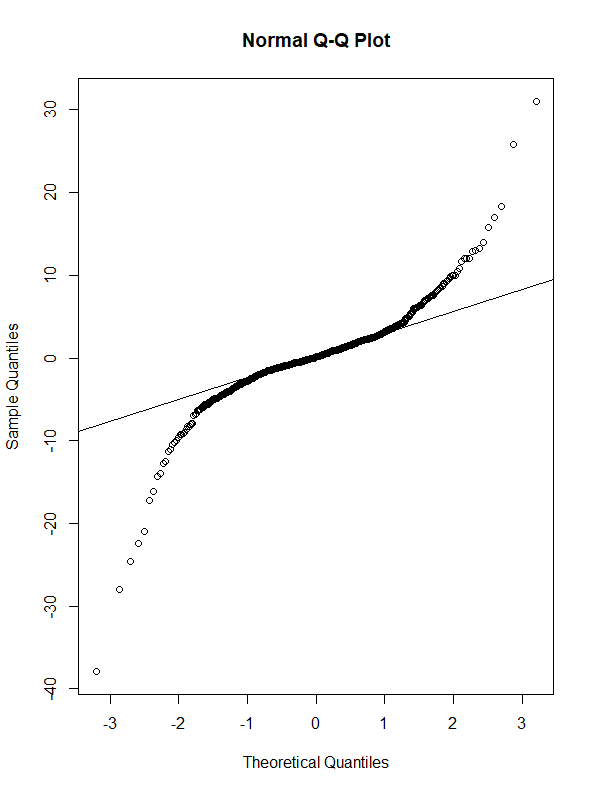
\includegraphics[height=2in]{ethqqbefno.png}
\caption{ Residual QQ plot for Ethereum during before period with no penalty}
  \end{subfigure}
% \begin{figure}[h]
  \begin{subfigure}{.49\textwidth}
  \centering

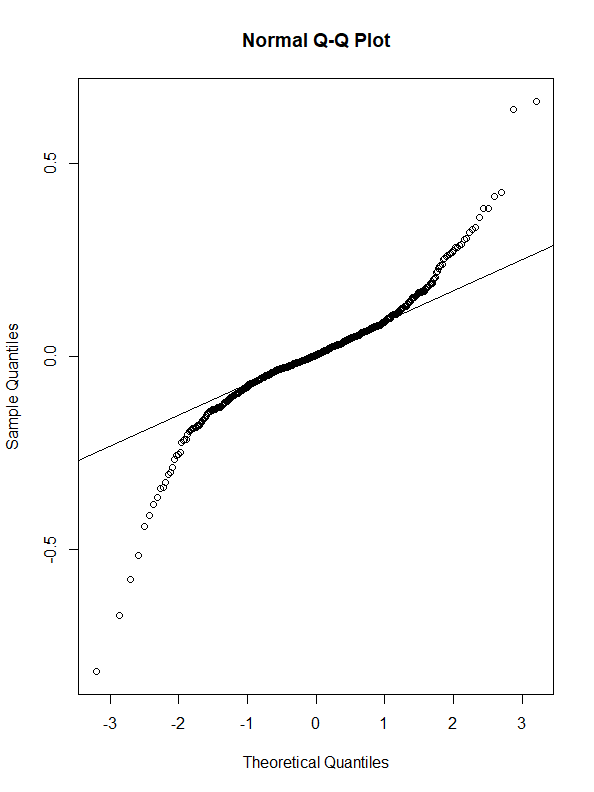
\includegraphics[height=2in]{ethqqbefstrong.png}
\caption{ Residual QQ plot for Ethereum during before period with strong penalty
}
\end{subfigure}
\caption{Residual QQ plot for Ethereum}
\end{figure}

\begin{landscape}
\begin{figure}[h!]
  \caption{Other Parameters}
  \centering
  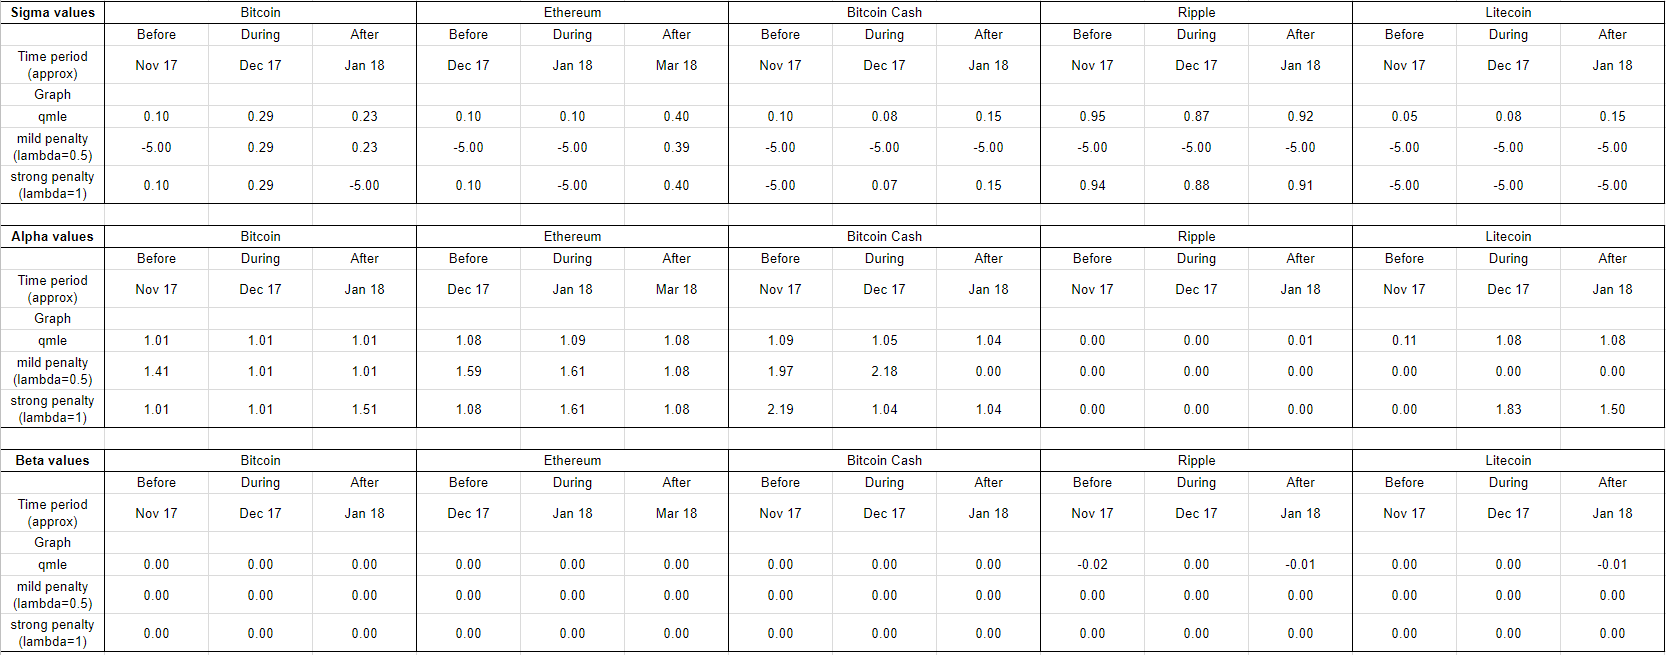
\includegraphics[width=1.4\textwidth]{greeks.PNG}
\end{figure}

\end{landscape}

\end{spacing}
\end{document}